% ===================================================================
% Arquivo: capitulos/parte-III-pilares/cap-08-retificadoras.tex
% ===================================================================

\chapter{Funções de Ativação Retificadoras}
\label{cap:ativacao-retificadoras}

\begin{flushright}
\textit{"caramba! A perda do meu modelo está em 31.415"} \\
--- Estagiário conhecendo o problema dos gradientes explosivos
\end{flushright}

No Capítulo \ref{cap:ativacao-sigmoidais} foi apresentado as funções de ativação sigmoidais. Essas funções estiveram presentes em um grande quantidade de redes neurais criadas até os anos 2010, sendo consideradas padrões para se utilizarem ao construir uma RNA. Contudo, essas funções são susceptíveis ao problema do desaparecimento do gradiente, um problema que afetou consideravelmente como as redes neurais eram construídas ao utilizar esse tipo de função de ativação, pois não era possível construir redes muito profundas.

Nesse cenário surgem as funções retificadoras, como uma solução para contornar esse problema. Essas funções são o tópico central desse capítulo. Para isso, primeiro será vista a \textit{rectfied linear unit}, também conhecida como \textit{ReLU}, conhecendo as suas origens, propriedades, fórmulas e como ela permitiu a criação de redes neurais mais profundas. Em seguida, será visto um problema crônico dessa função de ativação: os \textit{ReLUs} agonizantes.

Para contornar esse problema, surgem então variantes da \textit{ReLU} com vazamento, permitindo que um pouco de gradiente flua pela rede para os casos em que a entrada dessa função seja negativa. Serão vistas nessa seção três funções: a \textit{Leaky ReLU}, a \textit{Parametric ReLU}, e a \textit{Randomized Leaky ReLU}. Seguindo adiante serão vistas também variantes que apresentam curvas suaves em seus gráficos, como a \textit{ELU} e a \textit{SELU}. Para todas essas funções serão apresentados diversos comparativos para entender melhor o seu desempenho e em quais cenários elas são ideais.

Essas funções também não são perfeitas, assim como a sigmoidais, elas também acabaram por introduzir uma nova classe de problemas. Neste caso, um problema que pode ocorrer ao se utilizar uma função retificadora é o do chamado gradiente explosivo, que, assim como o desaparecimento do gradiente, impede o aprendizado dos neurônios da rede. O capítulo termina com uma tabela, compilando as principais características dessa família de funções de ativação.

% ===================================================================
% Resumo do capítulo
% ===================================================================

\section{Exemplo Ilustrativo: Vendendo Pipoca}

Imagine que você está querendo ganhar dinheiro e decidiu vender pipoca em uma praça da sua cidade. Você comprou milho, óleo, sal e manteiga, um carrinho para poder levar e fazer as pipocas, além disso, você também comprou vários pacotes para poder colocar as pipocas para vender.

Nisso, você teve que estipular um valor para vender essas pipocas, após pensar um pouco e analisar todos os seus gastos, você estimou que um valor de R\$ 5,00 seria ideal, pois conseguiria pagar os seus gastos mas você ainda ia obter lucro dos seus clientes.

Agora você está pronto para vender, começou a fritar o milho e colocou uma plaquinha com o preço ao lado do seu carrinho. Então chega uma pessoa com R\$ 6,00 e decide comprar um pacote, você vende e entrega um real de troco. Logo em seguida aparece uma segunda pessoa com R\$ 4,99 e decide negociar com você, ela afirma que é quase R\$ 5,00, e por isso, você deveria vender a pipoca para ela, mas você explica que só vende pelo valor de R\$ 5,00.

Com base nisso, nós podemos chegar em uma situação em que um pacote de pipoca será vendido somente se uma pessoa possuir R\$ 5,00 no bolso, ou mais. Podemos então escrever algo como o da equação \ref{eq: VendaPipoca}. Em casos em que uma venda ocorre, você poderá vender mais um pacote, para isso, o seu comprador deverá possuir pelo menos R\$ 10,00, assim, $x$ que indica a quantidade de pacotes vendido seguirá a lei de formação $x = 5 \mod d$, em que $d$ é o dinheiro que a pessoa possui.

\begin{equation}
    \text{Número de Pacotes} = \begin{cases} 0 & \text{quando } R\$ \leq  4,99 \\ x & \text{quando } R\$ > 4,99 \end{cases}
    \label{eq: VendaPipoca}
\end{equation}

Saindo do assunto da pipoca e voltando para o tema deste texto, existe uma família de funções de ativação que funciona de forma semelhante a lógica de venda dos pacotes de pipoca, elas são as unidades lineares retificadoras. A ReLU, que dá nome a essa família, funciona de forma semelhante a essa venda, ela tem um comportamento de "tudo ou nada", em que irá comandar quando um neurônio de uma rede neural irá disparar seu resultado.

% ===================================================================
% ReLU
% ===================================================================

\section{Rectified Linear Unit (ReLU): A Revolução Retificadora}

Como foi visto anteriormente no Capítulo \ref{cap:ativacao-sigmoidais}, as funções sigmoidais surgiram com inspiração nos neurônios humanos e como eles se comportam com determinados estímulos. Mas essas não foram as únicas funções que tiveram essa origem. Na década de 40, o pesquisador Alton Householder estava estudando um cenário parecido em seu trabalho \textit{A theory of steady-state activity in nerve fiber network: I. Definition of mathematical biofysics}, nele o autor analisou o comportamento de fibras nervosas e quando elas irão assumir caráter excitatório ou inibitório, para isso ele apresentou a Equação \ref{eq:fibra-nervosa-householder} \parencite{Householder1941}.

\begin{equation}
    a_{ij} = \begin{cases} 0 & \text{quando } \eta_i \le h_{ij} \\ a_{ij}, & \text{quando } \eta_i > h_{ij} \end{cases}
    \label{eq:fibra-nervosa-householder}
\end{equation}

Essa equação mostra quando uma fibra nervosa irá disparar, para isso, deve-se olhar o limiar da fibra $h_{ij}$ e o estímulo total $\eta_i$, com base nesses valores e no que a fórmula apresenta, uma fibra irá disparar quando o estímulo total for maior que o seu limiar, quando isso não ocorrer, ela não irá disparar \parencite{Householder1941}. Além disso, \textcite{Householder1941} explica também sobre o termo $a_{ij}$, a saída dessa função, segundo o autor ele é utilizado para representar o parâmetro de atividade, sendo um valor diferente de zero, podendo ser positivo (quando a fibra possui ação excitatória), ou negativo (apresentando caráter inibitório).

Essa equação criada por Householder, lembra bastante a expressão da função \textit{ReLU}, a qual é denotada pelas Equações \ref{eq:relu}.

\begin{equacaodestaque}{\textit{Rectified Linear Unit} (\textit{ReLU})}
    \mathcal{A}_{\text{ReLU}}(y_j) = \begin{cases}y_j, & \text{se } y_j > 0 \\0, & \text{se } y_j \leq 0\end{cases} \quad \text{ou} \quad \mathcal{A}_{\text{ReLU}}(y_j) = \max(0, y_j)
    \label{eq:relu}
\end{equacaodestaque}

Dito isso, mesmo com ela existindo a mais de 80 anos, ela só passou a ser amplamente utilizada nos anos 2010, antes disso, as sigmoides eram a grande maioria quando o assunto era função de ativação. Contudo, as sigmoides eram funções saturantes, e isso fazia com que sua derivada retornasse muitos valores pequenos ao longo da função. Ao multiplicar vários valores pequenos na retropropagação do gradiente, o vetor gradiente ia diminuindo até chegar um ponto em que ele não conseguia atualizar os pesos e vieses das redes neurais de forma eficiente, assim, tínhamos o problema do desaparecimento do gradiente. As funções retificadoras, sendo a principal delas a \textit{ReLU}, surgem para corrigir esse problema crônico. 

Dessa forma, antes de conhecer de fato a \textit{ReLU} e suas propriedades, é preciso entender o cenário que ela se popularizou, com os cientistas buscando novos tipos de funções de ativação que substituísse as sigmoides, funções saturantes, por outro tipo de função que resolvesse o problema do desaparecimento do gradiente.

Nesse cenário, artigos como \textit{Rectified Linear Units Improve Restricted Boltzmann Machines} foram essenciais para popularizar a \textit{ReLU} como uma função de ativação interessante para se utilizar em redes neurais. No trabalho, \textcite{Nair2010} foram responsáveis por demonstrar propriedades úteis das funções retificadoras, como a capacidade da \textit{NReLU} de auxiliar em reconhecimentos de objetos por possuir equivariância de intensidade(\textit{intensity equivarience}), o que significa que se a intensidade da entrada de uma função for alterada por um determinado fator a intensidade de sua saída será alterada pelo mesmo fator. Essa propriedade se torna bastante útil em casos que queremos preservar informações, como ao comparar imagens, garantindo melhor precisão por exemplo em situações de baixa luz quando comparados com cenários em que possuem muita luz nas imagens.

Além disso, no trabalho \textit{Deep Sparse Rectifier Neural Networks} dos autores \textcite{Glorot}, o uso de unidades retificadoras não lineares são propostos como alternativas para a tangente hiperbólica e sigmoide em redes neurais profundas, mas também os pesquisadores são capazes de demonstrar que as unidades retificadoras se aproximam melhor do comportamento de neurônios biológicos. Um ponto chave desse texto é que os autores destacam características importantes que a esparsidade traz para uma rede neural possibilitada pelo uso de funções retificadoras \parencite{Glorot}. Entre elas estão:

\begin{itemize}
    \item \textbf{Desembaraçamento de Informações:} Um dos principais objetivos dos algoritmos de aprendizado profundo é desembaraçar os fatores que explicam as variações nos dados, assim, existem diferentes tipos de representações, uma representação densa é altamente emaranhada porque quase qualquer mudança na entrada modifica a maior parte as entradas no vetor de representação, contudo, se tivermos uma representação esparsa e robusta a pequenas mudanças na entrada, o conjunto de características diferentes de zero é quase sempre aproximadamente conservado por pequenas mudanças na entrada \parencite{Glorot};
    \item \textbf{Representação eficiente de tamanho variável}. Diferentes entradas podem conter diferentes quantidades de informação e seriam mais convenientemente representadas usando uma estrutura de dados de tamanho variável, o que é comum em representações computacionais de informação, assim é interessante poder variar o número de neurônios ativos permitindo que um modelo controle a dimensionalidade efetiva da representação para uma determinada entrada e a precisão necessária \parencite{Glorot};
    \item \textbf{Separabilidade linear}. Representações esparsas também são mais propensas a serem linearmente separáveis, ou mais facilmente separáveis com menos maquinário não linear, simplesmente porque a informação é representada em um espaço de alta dimensão, além disso, isso pode refletir o formato original dos dados \parencite{Glorot};
    \item \textbf{Distribuídas, mas esparsas}. Representações densamente distribuídas são as representações mais ricas, sendo potencialmente exponencialmente mais eficientes do que as puramente locais, além disso a eficiência das representações esparsas ainda é exponencialmente maior, com a potência do expoente sendo o número de características diferentes de zero, elas podem representar uma boa compensação em relação aos critérios acima \parencite{Glorot}.
\end{itemize}

Por fim, um último trabalho que colaborou para a popularização da \textit{ReLU} foi a \textit{AlexNet}, de \textcite{AlexNet}, essa rede neural convolucional (\textit{CNN}) foi capaz ganhar o Desafio de Reconhecimento Visual em Larga Escala \textit{ImageNet} (\textit{ILSVRC}) sendo treinada para classificar 1.2 milhões de imagens de alta resolução e classificá-las em 1000 diferentes classes. Para isso, essa \textit{CNN} foi construída utilizando 8 camadas com pesos, sendo as primeiras 5 camadas convolucionais, enquanto as três últimas são camadas totalmente conectadas, a última camada de neurônios faz uso da função de ativação \textit{softmax} para fazer a distribuição em 1000 diferentes classes, por último mas não menos importante, a \textit{AlexNet} fez uso da ReLU em sua arquitetura \parencite{AlexNet}.

Assim, como pode ser visto na tabela \ref{tab:desempenho-alexnet}, a \textit{AlexNet} foi capaz de alcançar uma taxa de erro de 15.3\% na fase de testes, note com base na variação de camadas convolucionais, que essa é uma rede que se beneficia da sua profundidade, algo que provavelmente só foi capaz de ocorrer devido ao uso da \textit{ReLU} como função de ativação, por não gerar o problema do desaparecimento de gradientes como nas sigmoidais. Além disso, a rede \textit{SIFT + FVs} (\textit{Scale-Invariant Feature Transform + Fisher Vectors}) é mostrada na tabela como base de comparativo, perceba que a \textit{AlexNet} foi capaz de diminuir com mais de 10\% dos erros que essa rede gerava.

Além disso, o modelo \textit{SIFT + FVs} (\textit{Scale-Invariant Feature Transform + Fisher Vectors},) o qual é apresentado como base de comparação, apresenta uma taxa de erro de 26.2\%, um aumento de 10 pontos percentuais quando comparado com o melhor modelo da \textit{AlexNet} de 15.3\%.

\begin{table}[ht]
    \centering
    \begin{threeparttable}
        \caption{Comparação das Taxas de Erro no \textit{AlexNet}}
        \label{tab:desempenho-alexnet}
        \begin{tabular}{lccc}
            \toprule
            \textbf{Modelo} & \textbf{Top-1 (validação)} & \textbf{Top-5 (validação)} & \textbf{Top-5 (teste)} \\
            \midrule
            SIFT + FVs & -    & -      & 26.2\% \\
            1 CNN      & 40.7\% & 18.2\% & -      \\
            5 CNNs     & 38.1\% & 16.4\% & 16.4\% \\
            1 CNN\textsuperscript{a}      & 39.0\% & 16.6\% & -      \\
            7 CNNs\textsuperscript{a}     & 36.7\% & 15.4\% & \textbf{15.3\%} \\
            \bottomrule
        \end{tabular}
        
        \begin{tablenotes}[para] % Ambiente para as notas e fonte
            \small % Define o tamanho da fonte
            \item[] Nota: A tabela compara as taxas de erro de diferentes modelos nos conjuntos de validação e teste do \textit{ILSVRC-2012}. Os valores em negrito indicam o melhor resultado. \textsuperscript{a}Modelos que foram pré-treinados para classificar todo o conjunto de dados ImageNet 2011 Fall.
            \item[] Fonte: Adaptado de "ImageNet Classification with Deep Convolutional Neural Networks", por A. Krizhevsky, I. Sutskever, \& G. E. Hinton, 2012, \textit{Advances in Neural Information Processing Systems, 25}.
        \end{tablenotes}

    \end{threeparttable}
\end{table}

A definição da \textit{ReLU} pode ser interpretada como uma pergunta, ao receber um número como entrada a \textit{ReLU} questiona: "esse número é menor que zero?", se a resposta for sim, ela retorna como resultado o número zero, se a resposta for não, ela irá retornar o próprio número como sua saída. Neste caso estão sendo considerados números, mas a analogia utilizada no início do texto em que o pacote de pipoca só é vendido caso a pessoa tenha mais de R\$ 5,00 também pode ser utilizada, em que o resultado seria um valor booleano, indicando se a pessoa vende ou não a pipoca.

Além de sua fórmula, é possível plotar o seu gráfico, que está presente na Figura \ref{fig:relu}, ele é bem mais simples quando comparado com a sigmoide, por exemplo, sendo apenas a junção de duas retas, uma delas uma função constante que irá retornar sempre zero e a outra a função identidade. Essa simplicidade da \textit{ReLU} é algo muito atrativo para os desenvolvedores, pois, ao utilizá-la ao invés de uma função mais complexa como a sigmoide ou a tangente hiperbólica, estamos diminuindo a complexidade da rede neural, se essa rede se torna mais simples, a tendência é de que ela possua um custo de poder de processamento menor permitindo que um volume maior de dados seja processado em menos tempo e com isso seu tempo de treinamento seja menor. Note que, antes da \textit{ReLU} surgir, muitos das funções de ativação faziam uso de exponenciais, a \textit{ReLU} não só resolvia o problema do desaparecimento do gradiente mas também era muito mais "barata".

\begin{figure}{h!}
    \centering
    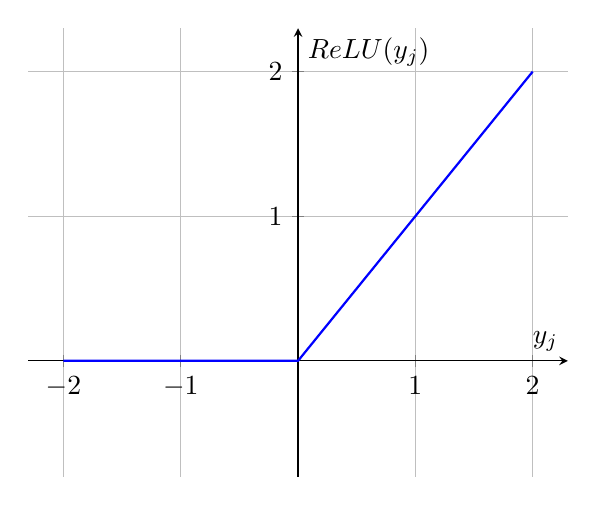
\begin{tikzpicture}
        \begin{axis}[
            xlabel={$y_j$},
            ylabel={$\text{ReLU}(y_j)$},
            xmin=-2.3, xmax=2.3,
            ymin=-0.8, ymax=2.3,
            axis lines=middle,
            grid=major,
        ]
        \addplot[blue, thick, domain=-2:2] {max(0, x)};
        \end{axis}
    \end{tikzpicture}
    \caption{Gráfico da função de ativação \textit{Rectified Linear Unit} (\textit{ReLU}).}
    \label{fig:relu}
    \fonte{O autor (2025).}
\end{figure}

ao trabalhar com redes neurais, uma das maiores vantagens destas é o fato de “aprenderem” com base na retropropagação do gradiente nas camadas da rede. Assim, ao calcular o gradiente para fazer a retropropagação do erro e ajustar os pesos e vieses das camadas, é necessário ter em mente também a derivada daquela função de ativação que que será aplicada em uma camada de neurônios da rede, dado que ela entrará no \textit{backward pass} do modelo.

Para achar a derivada da \textit{ReLU}, deve-se derivar as duas condicionais dela, assim, quando $x$ for maior que zero, a saída será 1, já quando $x$ for menor que zero, a saída será zero. Mas você vai encontrar um problema nisso, a derivada dessa função não existe quando $x$ é 0, pois o limite lateral à esquerda dessa função é zero, enquanto o limite lateral a direita dela é um. Isso passa a ser um problema quando queremos calcular o valor de saída justamente quando aquele valor de entrada é zero. Na prática, esse problema é fácil de resolver, ao desenvolver o código dessa função, escolher qual será o resultado da \textit{ReLU} quando esse valor de entrada for zero. Podemos dizer que ele será um ou zero, isso irá depender somente da nossa implementação da derivada da \textit{ReLU}.

Assim, a derivada da \textit{ReLU} é dada pela Equação \ref{eq:relu-derivada}.

\begin{equacaodestaque}{\textit{Rectified Linear Unit} (\textit{ReLU} Derivada)}
    \frac{d}{dy_j} [\mathcal{A}_{ReLU}](y_j) = \begin{cases}1, & \text{se } y_j > 0 \\0, & \text{se } y_j \leqslant 0 \end{cases}
    \label{eq:relu-derivada}
\end{equacaodestaque}

Esse detalhe da descontinuidade da \textit{ReLU} no ponto zero foi algo que acabou mudando em funções futuras, que buscam corrigir erros da \textit{ReLU} e melhorá-la, assim, com o passar do tempo foram surgindo outras alternativas que também trabalhassem com os atributos da ReLU, mas que fossem contínuas em toda a reta, permitindo a sua derivação também em todos os pontos. Uma dessas funções a \textit{ELU}, ela será explicada mais em frente.

Além da sua representação em forma de equação, é possível fazer também o seu gráfico na Figura \ref{eq:relu-derivada}, note que ele é ainda mais simples que a própria função de ativação, são só duas retas constantes que irão retornar zero quando o número for menor que zero, ou irão retornar 1 quando a entrada for um número maior que zero.

\begin{figure}[h!] % Use [htbp] para dar flexibilidade ao LaTeX
    \centering % Centraliza o gráfico na página
    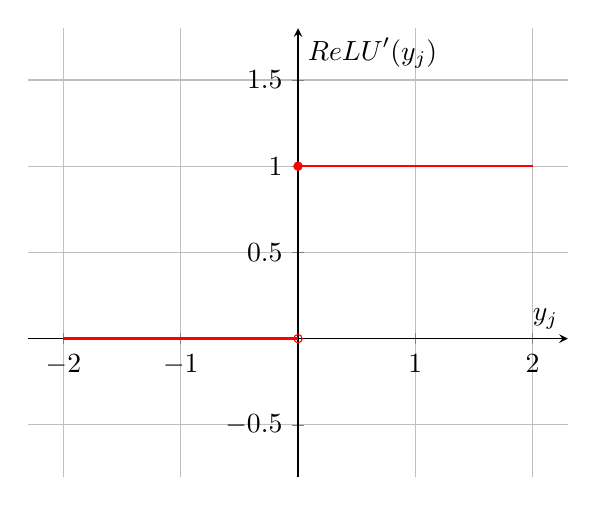
\begin{tikzpicture}
        \begin{axis}[
            xlabel={$y_j$},
            ylabel={$\text{ReLU}'(y_j)$},
            xmin=-2.3, xmax=2.3,
            ymin=-0.8, ymax=1.8,
            axis lines=middle,
            grid=major
        ]
        \addplot[red, thick, domain=-2:0] {0};
        \addplot[red, thick, domain=0:2] {1};
        \addplot[red, only marks, mark=o, mark size=1.5pt] coordinates {(0,0)};
        \addplot[red, only marks, mark=*, mark size=1.5pt] coordinates {(0,1)};
        \end{axis}
    \end{tikzpicture}
        \caption{Gráfico da derivada da função de ativação Rectified Linear Unit (ReLU).}
    \label{fig:relu-derivada}
    \fonte{O autor (2025).}
\end{figure}

\medskip
\begin{center}
 * * *
\end{center}
\medskip

\textbf{Algumas Aplicações da Rectified Linear Unit em Redes Neurais}
\vspace{1em}

\begin{itemize}
    \item \textbf{Aplicação 1 (Área):}
    \item \textbf{Aplicação 2 (Área):}
    \item \textbf{Aplicação 3 (Área):}
    \item \textbf{Aplicação 4 (Área):}
\end{itemize}

\medskip
\begin{center}
 * * *
\end{center}
\medskip

Assim, com toda essa simplicidade e versatilidade, a \textit{ReLU} se tornou uma função que é considerada padrão para a maioria das redes neurais \textit{feedforward} \parencite{DeepLearningBook}. Contudo, ela também apresenta problemas assim como as sigmoidais, sendo um desses problemas o dos \textit{ReLUs} agonizantes, o qual será explicado em sequência.

\section{O Problema dos ReLUs Agonizantes}

Mesmo apresentando tantas propriedades úteis, como o fato de impedir o problema do desaparecimento de gradientes além de ser uma função computacionalmente barata, a \textit{ReLU} não é perfeita. Ela é responsável por causar um problema conhecido como \textit{ReLUs} agonizantes (\textit{Dying ReLUs problem}), que será explicado nessa seção. Para isso, é preciso lembrar primeiro da equação da camada densa:

\[
    y = W^T  X + b
\]

Imagine que a \textit{ReLU} é a função de ativação que está sendo utilizada para introduzir a não-linearidade após essa camada, quando uma variável $y$ passar para uma função $\max(0, y)$, e condição mais comum dessa comparação for os casos em que $y < 0$ isso pode afetar negativamente o aprendizado do modelo na etapa do \textit{backward pass}, uma vez que a derivada será utilizada nessa parte, ela também será zero para os casos em que $y < 0$, e como foi visto no capítulo \ref{cap:retropropagacao-gradiente}, a derivada será utilizada para a multiplicação do gradiente, se a derivada é zero, o gradiente também é zero, e se o gradiente é zero, isso resulta em cenários nos quais os neurônios não vão ter seus pesos atualizados e portanto não irão aprender \parencite{DyingReluDouglas}. Como explica \textcite{DyingReluDouglas}, os neurônios irão morrer, passando apenas a retornar zeros independente de sua entrada.

Essa condição de vários neurônios morrendo causada pela \textit{ReLU} acabou por gerar um novo conjunto de funções, as quais possuem propriedades comuns da \textit{ReLU}, como a não linearidade e a simplicidade nos cálculos mas que buscam resolver ou amenizar esse problema em uma rede neural. Uma das funções que busca resolver esse problema é a \textit{Leaky ReLU} \parencite{DyingReluDouglas}.

\section{As Variantes com Vazamento: Corrigindo o Problema do ReLUs agonizantes}

Diferente da \textit{ReLU} tradicional que retorna zero para os casos em que sua entrada é negativa e por isso na sua derivada irá também retornar zero nestes casos, as variantes com vazamento atuam de outra forma, elas retornam um valor muito pequeno como 0.1, multiplicado pela entrada da função quando ela é negativa. Por isso, a sua derivada será algo também 0.1 (ou valores muito pequenos), isso permite um "vazamento" do gradiente em cenários nos quais a entrada do neurônio será negativa.

Como foi visto, que a causa do \textit{ReLUs} agonizantes era justamente isso: muitas situações em que a entrada era negativa, que gerava um gradiente nulo e consequentemente impedia os neurônios de terem seus pesos e vieses ajustados, e futuramente morrendo, retornando zero independente de qual fosse a sua entrada.

Assim, essas variantes, como a \textit{Leaky ReLU} e a \textit{PReLU} buscam tentar corrigir um amenizar esse problema da \textit{ReLU} mas mantendo algumas de suas principais propriedades, como a não linearidade, a capacidade de ser escrita compondo duas retas permitindo a criação de uma função simples e rápida de ser computada em uma rede neural.

\subsection{Leaky ReLU (LReLU)}

Seguindo adiante, é possível analisar agora a \textit{Leaky ReLU}, ela é uma variante da \textit{ReLU} que foi criada com intuito de corrigir o problema do \textit{ReLUs} agonizantes. Assim como a \textit{ReLU}, que foi explicada com a analogia do vendedor de pipoca, é possível extender essa explicação para essa nova função, antes o limiar para comprar um pacote de pipoca era de R\$ 5,00, quem tivesse menos que isso não comprava nada. Mas agora, para garantir que todos possam comprar pipoca, você como vendedor definiu que quando uma pessoa tiver menos que R\$ 5,00 ela também será capaz de comprar pipoca, só que neste caso ela comprará um punhado de pipoca que será proporcional ao dinheiro que ela tem multiplicado por uma constante $\alpha$. Assim, uma pessoa com um valor próximo de R\$ 5,00 pode sair com um punhado de pipoca quase igual ao do pacote original se essa constante $\alpha$ for um valor muito proximo de um. Com isso, você como vendedor consegue obter lucro com uma nova clientela além de não perder clientes por não possuírem o valor total do pacote de pipoca. A \textit{Leaky ReLU} traz uma proposta parecida para resolver com o problema do \textit{ReLUs} agonizantes.

Essa função de ativação foi apresentada no artigo \textit{Recfier Nonlinearites Improve Neural Networks Acustic Models}, em que os autores exploram o uso de redes retificadoras profundas como modelos acústicos para a tarefa de reconhecimento de fala conversacional \textit{switchboard} \parencite{LeakyReLUArticle}. Além disso, a sua principal diferença, como explicam \textcite{LeakyReLUArticle}, está no fato dela permitir que um pequeno gradiente diferente de zero flua quando a unidade está saturada e não ativa. Esse gradiente diferente de zero que flui quando a unidade está saturada e não ativa são os seus compradores de pipoca que não possuem o valor total mas são capazes de comprar um punhado dela, neste caso a unidade estará não ativa pois o valor de entrada é negativo mas irá retornar um valor diferente de zero, algo que não acontecia na \textit{ReLU}.

Também é possível discutir a expressão matemática da \textit{Leaky ReLU}, a qual é dada pela Equação \ref{eq:leaky-relu}, que é bem parecida com a \textit{ReLU}, porém, ela também irá retornar valores negativos quando a sua entrada for um valor negativo, diferente da \textit{ReLU}, que iria retornar como saída zero. A constante $\alpha$, no texto original é dada por 0.1 fazendo com que os valores negativos sejam pequenos mas ainda sim, diferentes de zero quando passam pela entrada \parencite{LeakyReLUArticle} \footnote{Cabe destacar que, essa constante $\alpha$ pode ser ajustada para diferentes cenários, podendo ser valores diferentes de 0.1 como foram propostos no texto original, é possível ver isso acontecendo em comparativos ao longo desse capítulo, em que diferentes autores optam por valores diferentes de $\alpha$ para melhor ajustar ao problema que está sendo analisado.}. 

\begin{equacaodestaque}{\textit{Leaky ReLU} (\textit{LReLU})}
    \mathcal{A}_{\text{LReLU}}(y_j) = \begin{cases}y_j, & \text{se } y_j \ge 0 \\ \alpha \cdot y_j, & \text{se } y_j < 0\end{cases} \quad \text{ou} \quad \mathcal{A}_{\text{LReLU}}(y_j) = \max(0, \alpha y_j)
    \label{eq:leaky-relu}
\end{equacaodestaque}

Em que a constante $\alpha$ representa uma constante pré-definida pelo programador ao desenvolver a rede neural. Por padrão, em bibliotecas como o \textcite{PyTorchLeakyReLU} essa constante tem valor de 0.1.

Já para a sua representação gráfica, ela está presente na Figura \ref{fig:leaky-relu}. Perceba que a \textit{Leaky ReLU} possui características muito semelhantes com a \textit{ReLU}, como o fato dela assumir o comportamento de uma função identidade para para valores positivos em sua entrada, mas, quando é analisado os seus valores negativos é possível ver uma diferença, agora eles são dados por um gráfico de uma função do primeiro grau, diferente da \textit{ReLU} que era uma função constante em zero. Além disso, a \textit{LReLU}, também é uma função assimétrica e não linear, bem como apresenta um ponto de descontinuidade em zero, pois ao traçar os seus limites laterais, eles apresentam valores diferentes, por isso ela não pode ser derivada nesse ponto, assim como a \textit{ReLU} vista anteriormente.

\begin{figure}[h!]
    \centering
    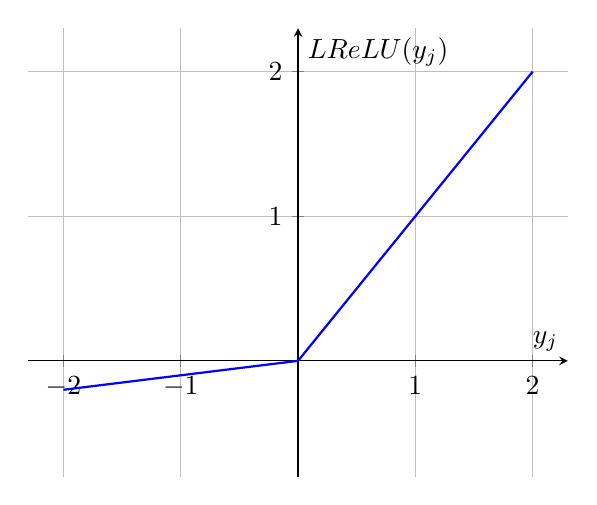
\begin{tikzpicture}
        \begin{axis}[
            xlabel={$y_j$},
            ylabel={$\text{LReLU}(y_j)$},
            xmin=-2.3, xmax=2.3,
            ymin=-0.8, ymax=2.3,
            axis lines=middle,
            grid=major,
        ]
        % \leakyalpha é o comando que você definiu no preâmbulo (0.1)
        \addplot[blue, thick, domain=-2:2] {x > 0 ? x : 0.1*x};
        \end{axis}
    \end{tikzpicture}
    \caption{Gráfico da função de ativação \textit{Leaky ReLU} (\textit{LReLU}) com $\alpha = 0.1$.}
    \label{fig:leaky-relu}
    \fonte{O autor (2025).}
\end{figure}

Sabendo de sua expressão e seu gráfico, é possível agora calcular sua derivada, para isso, deve-se derivar as duas condicionais que estão na função da \textit{Leaky ReLU}. Assim, quando a entrada dessa função for maior que zero, essa função será $x$ que derivada é 1, já quando a entrada for menor que zero, a função será $\alpha x$, que quando derivada tem como resultado a própria constante $\alpha$. Contudo, como dito anteriormente, a derivada da \textit{Leaky ReLU} não existe quando a entrada é exatamente zero, mas na prática, ao trabalhar com a sua definição na retropropagação, é possível definir um valor para a derivada nesse ponto, assim como foi feito com a \textit{ReLU} tradicional. Com isso em mente, tem-se então a Equação \ref{eq:leaky-relu-derivada}, a qual representa a derivada da \textit{Leaky ReLU}.

\begin{equacaodestaque}{\textit{Leaky ReLU} (\textit{LReLU} Derivada)}
    \frac{d}{dy_j} [\mathcal{A}_{LReLU}](y_j) = \begin{cases}1, & \text{se } y_j > 0 \\ \alpha, & \text{se } y_j \leqslant  0 \end{cases}
    \label{eq:leaky-relu-derivada}
\end{equacaodestaque}

Já que a sua derivada é conhecida, pode-se também plotar o seu gráfico, o qual é dado pela figura \ref{fig:leaky-relu-derivada}. Ele também é parecido com o gráfico da \textit{ReLU} visto anteriormente, sendo composto por duas retas constantes, para valores positivos ele retorna 1 (assim como a \textit{ReLU}), e para valores negativos ou nulos ele irá sempre retornar a constante $\alpha$, diferente da \textit{ReLU}, que iria retornar zero, indicando que neste caso o neurônio não está passando nenhuma informação na na retropropagação do gradiente. Por esse motivo que e a \textit{Leaky ReLU} tem esse nome, pois \textit{leaky} em inglês significa "vazamento", e neste caso, como a derivada dela é diferente de zero, mesmo quando a entrada for negativa, ela irá passar informações durante a retropropagação, isso permite que o neurônio não morra, como acontecia em algumas redes que faziam uso da \textit{ReLU} tradicional, e por esse motivo continue aprendendo pelo fato do gradiente continuar fluindo pela rede e consequentemente atualizando os pesos e vieses dos neurônios.

\begin{figure}[h!]
    \centering
    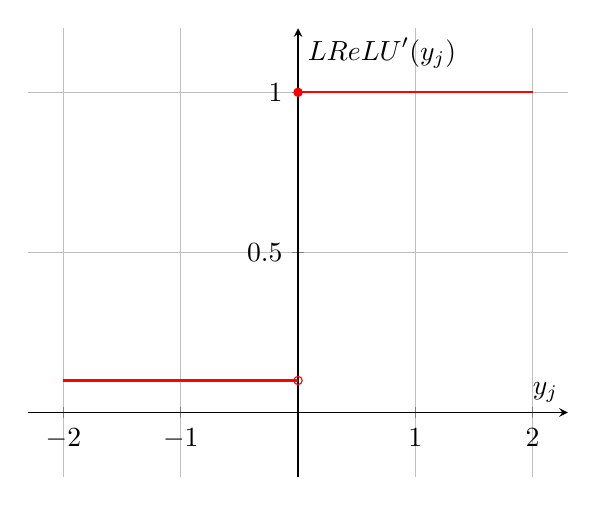
\begin{tikzpicture}
        \begin{axis}[
            xlabel={$y_j$},
            ylabel={$\text{LReLU}'(y_j)$},
            xmin=-2.3, xmax=2.3,
            ymin=-0.2, ymax=1.2,
            axis lines=middle,
            grid=major
        ]
        \def\alphaVal{0.1} % Define alpha for the derivative graph

        \addplot[red, thick, domain=-2:0] {\alphaVal};
        \addplot[red, thick, domain=0:2] {1};
        \addplot[red, only marks, mark=o, mark size=1.5pt] coordinates {(0,\alphaVal)};
        \addplot[red, only marks, mark=*, mark size=1.5pt] coordinates {(0,1)};
        \end{axis}
    \end{tikzpicture}
    \caption{Gráfico da derivada da função de ativação \textit{Leaky ReLU} (\textit{LReLU}) com $\alpha = 0.1$.}
    \label{fig:leaky-relu-derivada}
    \fonte{O autor (2025).}
\end{figure}

Conhecendo a \textit{leaky ReLU} e suas propriedades, é possível agora entender como essa função se comporta quando comparada com outras em testes.

Em testes de desempenho realizados por \textcite{LeakyReLUArticle} em seu trabalho, eles foram capazes de analisar como uma rede neural que faz uso dessa função pode performar quando comparada com a \textit{ReLU} tradicional e também com redes que fazem uso da tangente hiperbólica, esse comparativo pode ser visto na Tabela \ref{tab:leaky-relu-desempenho}. Note que as redes neurais que fizeram uso da \textit{Leaky ReLU} como função de ativação obtiveram melhores resultandos quando comparadas com as redes que utilizaram a \textit{ReLU} tradicional ou mesmo a tangente hiperbólica, veja que a rede que foi construída com 3 camadas utilizando a \textit{LReLU} foi capaz de obter a menor taxa de erro de palavra (\textit{WER}) no conjunto \textit{SWBD}, com 17.8\%, esse resultado 0.3 pontos percentuais menor quando comparado com uma mesma rede de três camadas que utilizou a \textit{ReLU} tradicional.

Além disso, ainda na tabela \ref{tab:leaky-relu-desempenho}, nas redes compostas por três camadas, a rede que fez uso da \textit{LReLU} também foi melhor que suas outras concorrentes que fizeram uso da \textit{ReLU} e da tanh, sendo capaz de ter a menor taxa de erro de palavra no conjunto de avaliação (\textit{EV}), com 24.3\%, uma diferença de 0.1 pontos percentuais quando comparada com a \textit{ReLU} de 24.4\%, já quando essa rede é comparada com a tangente hiperbólica, a diferença é ainda maior, sendo de 2.1 pontos percentuais, indicando que a \textit{LReLU} traz resultados melhores quando comparada com essas duas funções de ativação.

\begin{table}[ht]
    \centering
    \begin{threeparttable}
        \caption{Comparativo de Desempenho de Redes Neurais para Reconhecimento de Fala}
        \label{tab:leaky-relu-desempenho}
        \begin{tabular}{lccccc}
            \toprule
            \textbf{Modelo} & \textbf{Dev CrossEnt} & \textbf{Dev Acc (\%)} & \textbf{SWBD WER} & \textbf{CH WER} & \textbf{EV WER} \\
            \midrule
            
            GMM Baseline & N/A & N/A & 25.1 & 40.6 & 32.6 \\ 
            \addlinespace % Adiciona um espaço para separar o baseline dos outros
            2 Camadas Tanh  & 2.09 & 48.0 & 21.0 & 34.3 & 27.7 \\
            2 Camadas ReLU  & 1.91 & 51.7 & 19.1 & 32.3 & 25.7 \\
            2 Camadas LReLU & 1.90 & 51.8 & 19.1 & 32.1 & 25.6 \\ 
            \addlinespace
            3 Camadas Tanh  & 2.02 & 49.8 & 20.0 & 32.7 & 26.4 \\
            3 Camadas ReLU  & 1.83 & 53.3 & 18.1 & 30.6 & 24.4 \\
            3 Camadas LReLU & 1.83 & 53.4 & \textbf{17.8} & 30.7 & \textbf{24.3} \\ 
            \addlinespace
            4 Camadas Tanh  & 1.98 & 49.8 & 19.5 & 32.3 & 25.9 \\
            4 Camadas ReLU  & 1.79 & 53.9 & 17.3 & 29.9 & 23.6 \\
            4 Camadas LReLU & \textbf{1.78} & 53.9 & 17.3 & 29.9 & 23.7 \\
            
            \bottomrule
        \end{tabular}
        
        \begin{tablenotes}[para]
            \small
            \item[] Nota: Comparação de métricas de erro para sistemas de redes neurais profundas (DNN) em reconhecimento de fala. As métricas de quadro a quadro (frame-wise) foram avaliadas em um conjunto de desenvolvimento, e as taxas de erro de palavra (WER) no conjunto de avaliação Hub5 2000 e seus subconjuntos. Abreviações: Dev CrossEnt = Entropia Cruzada no conjunto de desenvolvimento; Dev Acc = Acurácia no conjunto de desenvolvimento; WER = Taxa de Erro de Palavra (Word Error Rate); SWBD = Switchboard; CH = CallHome; EV = Evaluation set. Valores em negrito indicam os melhores resultados para modelos de 3 e 4 camadas.
            \item[] Fonte: Adaptado de "Rectifier Nonlinearities Improve Neural Network Acoustic Models", por A. L. Maas, A. Y. Hannun, \& A. Y. Ng, 2013, \textit{In Proceedings of the 30th International Conference on Machine Learning, Workshop on Deep Learning for Audio, Speech and Language Processing}.
        \end{tablenotes}
        
    \end{threeparttable}
\end{table}

Agora comparando as redes que fazem uso de quatro camadas, cabe destacar os resultados da entropia cruzada no conjunto de desenvolvimento (\textit{Dev CrossEnt}), que é uma métrica responsável por medir a diferença entre duas distribuições de probabilidade, neste cenário: a distrubição de probabilidade prevista pelo modelo e a distribuição de probabilidade real, com base nesses dois valores, a entropia cruzada consegue medir o quão bem o modelo de rede neural criado pelos pesquisadores está prevendo a transcrição correta da fala durante a fase de treinamento e ajuste, para isso, é utilizado o conjunto de dados de desenvolvimento (\textit{Dev Set}). Tendo isso em mente, o modelo de quatro camadas que fez uso da \textit{Leaky ReLU} em sua arquitetura obteve o melhor resultado dos seus outros dois concorrentes, sendo assim, ele teve como resultado uma entropia cruzada de 1.78, 0.01 menor que o modelo que fez uso da \textit{ReLU} tradicional (que obteve 1.79) e 0.2 menor que o modelo que fez uso da tangente hiperbólica (que obteve 1.98).

Ainda no grupo de redes que possuem quatro camadas, é possível ver um empate ao analisar a acurácia no conjunto de desenvolvimento (\textit{Dev Acc}), que é uma métrica responsável por medir a proporção das previsões corretas feitas pelo modelo quando comparadas com o total de previsões feitas. Assim, perceba que na tabela \ref{tab:leaky-relu-desempenho}, as redes que fizeram uso tanto da \textit{ReLU} quanto da \textit{Leaky ReLU} obtiveram a mesma acurácia de 53.9\%, já quando comparadas com a tangente hiperbólica, é possível ver uma diferença de 4.1 pontos percentuais, indicando as funções retificadoras acabam sendo mais precisas para essa análise. Não somente elas são mais precisas, mas quando comparadas com a \textit{Leaky ReLU}, nota-se outros ganhos também, como menores taxas de erro de palavra (\textit{WER}) tanto no conjunto \textit{Switchboard} (\textit{SWBD}) quanto no conjunto de avaliação (\textit{EV}).

\medskip
\begin{center}
 * * *
\end{center}
\medskip

\textbf{Algumas Aplicações da Leaky ReLU em Redes Neurais}
\vspace{1em}

\begin{itemize}
    \item \textbf{Aplicação 1 (Área):}
    \item \textbf{Aplicação 2 (Área):}
    \item \textbf{Aplicação 3 (Área):}
    \item \textbf{Aplicação 4 (Área):}
\end{itemize}

\medskip
\begin{center}
 * * *
\end{center}
\medskip

Assim, a \textit{Leaky ReLU} já é uma evolução quando comparamos com a ReLU tradicional, mas, é possível ir além e encontrar funções ainda mais complexas que também buscam assim como a \textit{LReLU} resolver o problema dos \textit{ReLUs} agonizantes com um vazamento de gradiente nos casos negativos, uma dessas funções é a \textit{PReLU}, a qual será vista em seguida.

\subsection{Parametric ReLU (PReLU)}

Continuando nas analogias do vendedor de pipoca para explicar as funções retificadoras, podemos também pensar uma para a \textit{Parametric ReLU}. Na \textit{LReLU} nós tínhamos uma constante fixa, que valia para todos os valores de entrada e não mudava, era como se o vendedor de pipoca definisse um valor para a proporção de pipoca que a pessoa irá receber quando tiver com uma quantia menor de dinheiro que o limiar da venda. Mas agora, este vendedor está mais experiente, e sabe que pode ajustar essa constante sempre que quiser, assim, quando estiverem muitas pessoas na praça em que está vendendo pipoca, ele poderá colocar uma constante que será capaz de dar uma quantidade ainda maior de pipoca para aqueles que não possuem o valor total de um pacote, o que incentivaria a venda para as pessoas. Já quando estivesse em um lugar mais vazio, colocaria uma constante que daria menos pipoca, para maximizar o seu lucro. A Diferença da \textit{PReLU} para a \textit{LReLU} está justamente nessa constante e como ela irá se comportar.

Proposta por \textcite{PReLUArticle} no artigo \textit{Delving Deep into Rectifiers: Surpassing Human Level Performance on Image Net Classification}, a \textit{PReLU} surgiu como uma variação não somente da \textit{ReLU}, mas também uma evolução da \textit{Leaky ReLU} que foi vista anteriormente, isso ocorre, pois diferente da \textit{LReLU} que possuía uma constante $\alpha$ fixa que multiplicava o valor da entrada nos casos negativos, a \textit{PReLU} trás essa mesma constante, mas neste caso ela é adaptável, se ajustando as particularidades de cada problema que uma rede neural está tentando resolver. Assim, a \textit{PReLU} é como o pipoqueiro mais experiente, que ajusta como vai vender o seu punhado de pipoca em cada uma das situações para poder maximizar os seus lucros mas ao mesmo tempo garantir mais clientes para si.

A fórmula matemática da \textit{PReLU} é dada pela Equação \ref{eq:prelu}. Como explicam \textcite{PReLUArticle}, a \textit{PReLU} generaliza a tradicional \textit{ReLU}, além de melhorar o \textit{model fitting} apresentando quase nenhum custo computacional extra e com um baixo risco de sobreajuste (\textit{overfitting}). Este coeficiente $\alpha$, que ela apresenta assim como a \textit{Leaky ReLU} que foi visto anteriormente, é aprendível, e não uma constante fixa, isso indica ser otimizado utilizando a retropropagação do gradiente de forma simultânea com as outras camadas da rede neural criada \parencite{PReLUArticle}. Assim, por esse fato tem-se uma melhor eficiência no aprendizado e no tempo da rede, dado que não precisamos criar uma nova etapa só para ajustar os valores de \textit{alpha} das camadas densas que fazem o uso da \textit{Parametric ReLU}.

\begin{equacaodestaque}{\textit{Parametric ReLU} (\textit{PReLU})}
    \mathcal{A}_{\text{PReLU}}(y_j) = \begin{cases}y_j, & \text{se } y_j \ge 0 \\ \alpha_i \cdot y_j, & \text{se } y_j < 0\end{cases} \quad \text{ou} \quad \mathcal{A}_{\text{PReLU}}(y_j) = \max(0, \alpha y_j)
    \label{eq:prelu}
\end{equacaodestaque}

Com base em sua equação, tem-se o gráfico da \textit{PReLU} na Figura \ref{fig:prelu}, note que caso este coeficiente for igual a zero, nos temos então a \textit{ReLU} tradicional, já quando ele for igual a 0.1, tem-se a \textit{LReLU}, no gráfico $\alpha$ está com valor de 0.2, mas ele irá variar conforme a rede aprende e para cada problema, podendo apresentar diferentes valores em diferentes situações. Com isso, é possível perceber que a \textit{PReLU} é composta por duas funções do primeiro grau, sendo assimétrica, e também apresentando um ponto de descontinuidade em zero, o que impede de ser derivada neste ponto.

\begin{figure}[h!]
    \centering
    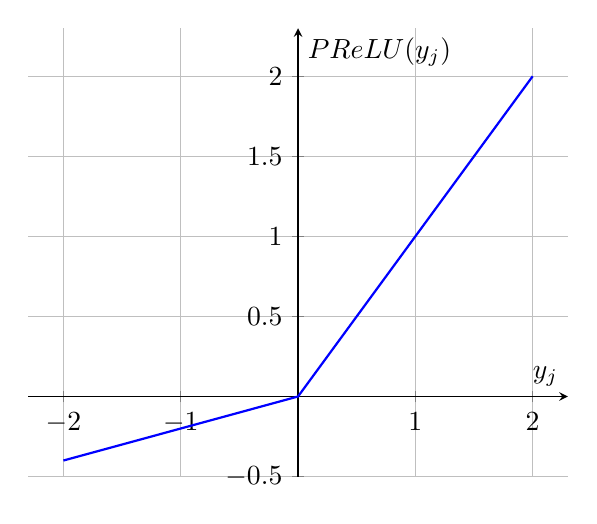
\begin{tikzpicture}
        \begin{axis}[
            xlabel={$y_j$},
            ylabel={$\text{PReLU}(y_j)$},
            xmin=-2.3, xmax=2.3,
            ymin=-0.5, ymax=2.3,
            axis lines=middle,
            grid=major,
        ]
        % Define um valor exemplo de alpha para o gráfico
        \def\alphaVal{0.2} 
        \addplot[blue, thick, domain=-2:2] {x >= 0 ? x : \alphaVal*x};
        \end{axis}
    \end{tikzpicture}
    \caption{Gráfico da função de ativação \textit{Parametric ReLU} (\textit{PReLU}) com $\alpha=0.2$.}
    \label{fig:prelu}
    \fonte{O autor (2025).}
\end{figure}

Conhecendo a sua fórmula e como ela se comporta, cabe também derivar a \textit{PReLU}, para isso, deve-se derivar cada uma das expressões dos condicionais de forma separada, assim como foi feito com a \textit{Leaky ReLU} e a \textit{ReLU} anteriormente. Como a fórmula da \textit{PReLU} é igual a \textit{LReLU}, podemos apenas nos lembrar dela e citar a Equação \ref{eq:prelu-derivada} como sua derivada. Note que, essa derivada também não existe quando a entrada é exatamente zero, mas assim como na \textit{Leaky ReLU}. É possível "corrigir" isso dizendo que ela será igual a $\alpha$ nesse ponto, para que o gradiente continue fluindo durante o \textit{backward pass}. Vale lembrar, que essa reta em $\alpha$ irá variar conforme a rede neural aprende as características e se ajusta ao problema que está tentando resolver.

\begin{equacaodestaque}{\textit{Parametric ReLU} (\textit{PReLU} Derivada)}
    \frac{d}{dy_j} [\mathcal{A}_{PReLU}](y_j) = \begin{cases}1, & \text{se } y_j > 0 \\ \alpha_i, & \text{se } y_j \le 0 \end{cases}
    \label{eq:prelu-derivada}
\end{equacaodestaque}

Sabendo a fórmula da derivada da \textit{PReLU}, é possível plotar o seu gráfico, o qual é dado pela Figura \ref{fig:prelu-derivada}, ele é semelhante ao gráfico da \textit{Leaky ReLU} visto na seção anterior, mas agora, a constante $\alpha$ está com valor em 0.2. Note que, o gráfico da derivada é também muito simples, sendo apenas duas funções constantes, uma que vale 1 para os valores de entrada positivos e outra que irá valer 0,2 para os outros valores. Assim, a \textit{PReLU} consegue manter a simplicidade da \textit{ReLU}, mas ao mesmo tempo fazendo pequenos ajustes garantindo melhorias de desempenho em redes mais profundas, como as que foram apresentas por \textcite{PReLUArticle}.

\begin{figure}[h!]
    \centering
    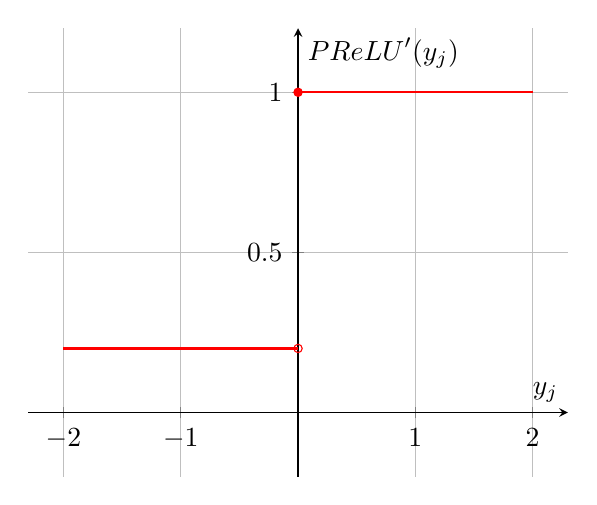
\begin{tikzpicture}
        \begin{axis}[
            xlabel={$y_j$},
            ylabel={$\text{PReLU}'(y_j)$},
            xmin=-2.3, xmax=2.3,
            ymin=-0.2, ymax=1.2,
            axis lines=middle,
            grid=major
        ]
        % Define um valor exemplo de alpha para o gráfico
        \def\alphaVal{0.2}

        \addplot[red, thick, domain=-2:0] {\alphaVal};
        \addplot[red, thick, domain=0:2] {1};
        \addplot[red, only marks, mark=o, mark size=1.5pt] coordinates {(0,\alphaVal)};
        \addplot[red, only marks, mark=*, mark size=1.5pt] coordinates {(0,1)};
        \end{axis}
    \end{tikzpicture}
    \caption{Gráfico da derivada da função de ativação \textit{Parametric ReLU} (\textit{PReLU}) com $\alpha=0.2$.}
    \label{fig:prelu-derivada}
    \fonte{O autor (2025).}
\end{figure}

Ainda em \textit{Delving Deep into Rectifiers: Surpassing Human Level Performance on Image Net Classification}, os autores realizam testes comparando a \textit{ReLU} tradicional com a \textit{PReLU} utilizando como base o \textit{dataset} de 1000 classes do \textit{ImageNet} 2012, o qual contêm cerca de 1.2 milhões de imagens de treino, 50.000 imagens de validação e 100.000 imagens de teste sem rótulos publicados \parencite{PReLUArticle}. Para isso, \textcite{PReLUArticle} criaram três modelos diferentes (A, B e C), baseados na arquitetura \textit{VGG-16} mas com variações entre si como diferentes números de camadas convolucionais e consequentemente complexidades distintas para cada algoritmo. Esses modelos podem ser vistos na Tabela \ref{tab:arquitetura-prelu}. 

\begin{table}
    \centering
    \begin{threeparttable}
        \caption{Arquiteturas dos modelos grandes}
        \label{tab:arquitetura-prelu}
        \begin{tabular}{cllll}
            \toprule
            \textbf{Input Size} & \textbf{VGG-19 [25]} & \textbf{Model A} & \textbf{Model B} & \textbf{Model C} \\
            \midrule
            224
              & \makecell[l]{3$\times$3, 64 \\ 3$\times$3, 64 \\ \addlinespace 2$\times$2 maxpool, /2}
              & 7$\times$7, 96, /2
              & 7$\times$7, 96, /2
              & 7$\times$7, 96, /2 \\
            \midrule
            112
              & \makecell[l]{3$\times$3, 128 \\ 3$\times$3, 128 \\ \addlinespace 2$\times$2 maxpool, /2}
              & 2$\times$2 maxpool, /2
              & 2$\times$2 maxpool, /2
              & 2$\times$2 maxpool, /2 \\
            \midrule
            56
              & \makecell[l]{3$\times$3, 256 \\ 3$\times$3, 256 \\ 3$\times$3, 256 \\ 3$\times$3, 256 \\ \addlinespace 2$\times$2 maxpool, /2}
              & \makecell[l]{3$\times$3, 256 \\ 3$\times$3, 256 \\ 3$\times$3, 256 \\ 3$\times$3, 256 \\ \addlinespace 2$\times$2 maxpool, /2}
              & \makecell[l]{3$\times$3, 256 \\ 3$\times$3, 256 \\ 3$\times$3, 256 \\ 3$\times$3, 256 \\ \addlinespace 2$\times$2 maxpool, /2}
              & \makecell[l]{3$\times$3, 384 \\ 3$\times$3, 384 \\ 3$\times$3, 384 \\ 3$\times$3, 384 \\ \addlinespace 2$\times$2 maxpool, /2} \\
            \midrule
            28
              & \makecell[l]{3$\times$3, 512 \\ 3$\times$3, 512 \\ 3$\times$3, 512 \\ 3$\times$3, 512 \\ \addlinespace 2$\times$2 maxpool, /2}
              & \makecell[l]{3$\times$3, 512 \\ 3$\times$3, 512 \\ 3$\times$3, 512 \\ 3$\times$3, 512 \\ \addlinespace 2$\times$2 maxpool, /2}
              & \makecell[l]{3$\times$3, 512 \\ 3$\times$3, 512 \\ 3$\times$3, 512 \\ 3$\times$3, 512 \\ \addlinespace 2$\times$2 maxpool, /2}
              & \makecell[l]{3$\times$3, 768 \\ 3$\times$3, 768 \\ 3$\times$3, 768 \\ 3$\times$3, 768 \\ \addlinespace 2$\times$2 maxpool, /2} \\
            \midrule
            14
              & \makecell[l]{3$\times$3, 512 \\ 3$\times$3, 512 \\ 3$\times$3, 512 \\ 3$\times$3, 512 \\ \addlinespace 2$\times$2 maxpool, /2}
              & \makecell[l]{3$\times$3, 512 \\ 3$\times$3, 512 \\ 3$\times$3, 512 \\ 3$\times$3, 512 \\ \addlinespace spp, \{7, 3, 2, 1\}}
              & \makecell[l]{3$\times$3, 512 \\ 3$\times$3, 512 \\ 3$\times$3, 512 \\ 3$\times$3, 512 \\ \addlinespace spp, \{7, 3, 2, 1\}}
              & \makecell[l]{3$\times$3, 896 \\ 3$\times$3, 896 \\ 3$\times$3, 896 \\ 3$\times$3, 896 \\ \addlinespace spp, \{7, 3, 2, 1\}} \\
            \midrule
            fc\textsubscript{1} & \multicolumn{4}{l}{4096} \\
            fc\textsubscript{2} & \multicolumn{4}{l}{4096} \\
            fc\textsubscript{3} & \multicolumn{4}{l}{1000} \\
            \midrule
            depth (conv+fc) & 19 & 19 & 22 & 22 \\
            complexity (ops., $\times 10^{10}$) & 1.96 & 1.90 & 2.32 & 5.30 \\
            \bottomrule
        \end{tabular}
        
        \begin{tablenotes}[para]
            \small
            \item[] Nota: Comparação detalhada das arquiteturas de rede. A notação "/2" denota um stride de 2. Cada coluna representa um modelo diferente. A tabela descreve a sequência de camadas convolucionais (no formato \texttt{kernel $\times$ kernel, n° de filtros}), de pooling e totalmente conectadas (fc). Os modelos A, B e C são variações da estrutura VGG-19, propostas pelos autores para avaliar a função de ativação PReLU. As linhas finais comparam a profundidade total (conv+fc) e a complexidade computacional de cada modelo.
            \item[] Fonte: Adaptado de "Delving Deep into Rectifiers: Surpassing Human-Level Performance on ImageNet Classification", por K. He, X. Zhang, S. Ren, \& J. Sun, 2015, \textit{Proceedings of the IEEE International Conference on Computer Vision (ICCV)}, pp. 1026-1034.
        \end{tablenotes}
        
    \end{threeparttable}
\end{table}

 Com isso, é possível ver na Tabela \ref{tab:prelu-desempenho} as métricas utilizadas pelos autores. É medido o erro \textit{Top-1} e o erro \textit{Top-5}, o erro \textit{Top-1} mostrando quão preciso é o modelo em seu melhor chute, já o erro \textit{Top-5} mostra se a resposta correta estava entre os top 5 melhores chutes feito pelo modelo. Assim, conhecendo esses parâmetros de medida, é possível chegar na conclusão de que quanto menor esses valores, melhor o modelo está performando, seguindo essa lógica, nota-se que todos os modelos que fazem uso de funções retificadoras, seja a \textit{PReLU} ou mesmo a \textit{ReLU} tradicional, são capazes de performar melhor que os modelos \textit{VGG-16} e \textit{GoogleLet} que fazem uso de outras funções de ativação.

\begin{table}[ht]
    \centering
    \begin{threeparttable}
        \caption{Resultados de Erro Top-1 e Top-5 no Conjunto de Validação ImageNet 2012}
        \label{tab:prelu-desempenho}
        \begin{tabular}{lcc}
            \toprule
            \textbf{Modelo} & \textbf{Erro Top-1 (\%)} & \textbf{Erro Top-5 (\%)} \\
            \midrule
            
            MSRA       & 29.68 & 10.95 \\
            VGG-16     & 28.07\textsuperscript{a} & 9.33 \\
            GoogleLeNet&  -    & 9.15 \\
            \addlinespace
            A, ReLU    & 26.48 & 8.59 \\
            A, PReLU   & 25.59 & 8.23 \\
            B, PReLU   & 25.53 & 8.13 \\
            C, PReLU   & \textbf{24.27} & \textbf{7.38} \\ 
            
            \bottomrule
        \end{tabular}
        
        \begin{tablenotes}[para]
            \small
            \item[] Nota: Resultados de erro (\%) para um único modelo com a técnica de 10-view no conjunto de validação do ImageNet 2012. Os modelos A, B e C são variações da arquitetura VGG-16 modificada pelos autores. Os valores em negrito indicam os melhores resultados. \textsuperscript{a}Resultado baseado em testes realizados pelos autores do artigo original.
            \item[] Fonte: Adaptado de "Delving Deep into Rectifiers: Surpassing Human-Level Performance on ImageNet Classification", por K. He, X. Zhang, S. Ren, \& J. Sun, 2015, \textit{Proceedings of the IEEE International Conference on Computer Vision (ICCV)}, pp. 1026-1034.
        \end{tablenotes}

    \end{threeparttable}
\end{table}

Ao comparar o modelo C, que faz uso da \textit{PReLU} e possui mais camadas convolucionais, com o modelo A que faz uso da \textit{ReLU}, é possível notar uma diferença de 2,21 pontos percentuais no erro \textit{Top-1}, já ao analisar o erro \textit{Top-5}, essa diferença é de 1,21 pontos percentuais, o que indica que a \textit{PReLU} é capaz de trazer melhores resultados quando comparada com redes que fazem uso da \textit{ReLU} tradicional. Já ao comparar com o \textit{VGG-16}, essa diferença de desempenho é ainda maior, sendo de 3,8 pontos percentuais no erro \textit{Top-1} e 1,95 pontos percentuais no erro \textit{Top-5}, note que a \textit{VGG-16}, a qual é indicada na Tabela \ref{tab:arquitetura-prelu} possui bem menos camadas convolucionais que o modelo C, é possível notar notar também a sua complexidade computacional, que é menos da metade da do modelo C, isso indica que a \textit{PReLU}, por ser uma função não saturante e consequentemente corrigir o problema do desaparecimento do gradiente, é capaz de criar redes neurais que se beneficiam melhor com uma maior profundidade, sendo capazes de extrair mais informações e com isso performar melhor.

Um feito importante que deve ser destacado sobre a \textit{PReLU}, que inclusive é o nome do artigo que foi responsável por introduzir essa função para a comunidade científica, é de que durante a pesquisa do texto \textit{Delving Deep into Rectifiers: Surpassing Human Level Performance on Image Net Classification}, \textcite{PReLUArticle} foram capazes de criar uma rede neural capaz de superar a capacidade humana de reconhecer diferentes conjuntos de imagens no \textit{ImagneNet} Classification, isso ocorreu porque a um humano ao analisar o \textit{ImageNet} apresenta uma taxa de erro \textit{Top-5} de 5.1\% e em um dos testes realizados pelos autores, uma rede neural alcançou uma taxa de erro \textit{Top-5} de 4.94\%, superando assim a capacidade humana de reconhecimento de imagens. 

Assim, é nítido destacar que não somente a \textit{PReLU}, mas as funções retificadoras de forma geral, foram capazes de trazer melhorias significativas para os modelos de aprendizado profundo quando comparadas com as funções sigmoides, as quais foram o padrão da indústria por muitos anos. De fato, a resolução do problema do desaparecimento do gradiente, possibilitou a criação de redes neurais ainda mais profundas, e com isso, sendo capazes de extrair mais informações e consequente melhores métricas, sendo capazes até de superar a capacidade humanas em algumas tarefas como no artigo de introdução da \textit{PReLU}.

\medskip
\begin{center}
 * * *
\end{center}
\medskip

\textbf{Algumas Aplicações da Parametric ReLU em Redes Neurais}
\vspace{1em}

\begin{itemize}
    \item \textbf{Aplicação 1 (Área):}
    \item \textbf{Aplicação 2 (Área):}
    \item \textbf{Aplicação 3 (Área):}
    \item \textbf{Aplicação 4 (Área):}
\end{itemize}

\subsection{Randomized Leaky ReLU (RReLU)}

Anteriormente, na \textit{Parametric ReLU}, existia uma padrão aprendível que era atualizado ao longo da retropropagação da rede, nós o comparamos com o caso do vendedor de pipoca ficando mais experiente para as vendas. No caso da \textit{RReLU} temos um vendedor um tanto quanto instável, ele se baseia na sorte/aleatoriedade para definir qual será o punhado de pipoca que cada pessoa irá receber ao comprar com um valor abaixo do limiar de venda. Para isso, não existe mais um padrão, algo como o horário ou a quantidade de pessoas na praça para fazer aumentar o diminuir a quantidade de pipoca que tera em um punhado. Essa estratégia parece caótica, mas pode ser interessante caso voce queira instigar as vendas e deixa-las divertidas, você pode comprar um punhado de pipoca, mas nao ira saber quanto irá receber, é uma grande aposta.

Segundo \textcite{XuRReLU}, em \textit{Empirical Evaluation of Rectified Activations in Convolutional Network}, a \textit{Randomized Leaky ReLU} foi proposta pela primeira vez em uma competição do \textit{Kaggle NDSB}, ela era uma função semelhante a \textit{leaky ReLU} mas que o seu coeficiente $\alpha$ é um número aleatório dado pela distribuição normal da forma $U(l, u)$, nessa mesma competição os valores escolhidos para essa distribuição foram de $U(3, 8)$.

A fórmula da \textit{RReLU} é dada pela Equação \ref{eq:rrelu}, note que é a mesma expressão da \textit{Leaky ReLU} e da \textit{PReLU}, mas o que muda é o significado do termo $\alpha$ em cada uma delas. Neste caso: $\alpha \sim U (l, u)$ em que $l < u$  e $l, u \in [0, 1)$ 

\begin{equacaodestaque}{\textit{Randomized Leaky ReLU} (\textit{RReLU})}
    \mathcal{A}_{\text{RReLU}}(y_j) = \begin{cases} y_j, & \text{se } y_j > 0 \\ \alpha_i y_j, & \text{se } y_j \leq 0 \end{cases} \quad \text{ou} \quad \mathcal{A}_{\text{RReLU}}(y_j) = \max(0, \alpha y_j)
    \label{eq:rrelu}
\end{equacaodestaque}

Na fase de testes, deve-se calcular a média de todos os valores de $\alpha$ durante o treino, e com isso $\alpha$ se torna uma constante fixa do tipo $(l+u)/2$ de forma que com isso seja possível obter um resultado determinístico, no artigo, os autores utilizam a fórmula \ref{eq:equacao-rrelu-teste} para calcular a \textit{RReLU} durante o teste do modelo \parencite{XuRReLU}.

\begin{equation}
    \mathcal{A}_{\text{RReLU}}(y_j) = \frac{y_j}{\frac{l + u}{2}}
    \label{eq:equacao-rrelu-teste}
\end{equation}

O gráfico da \textit{RReLU} está presente na Figura \ref{fig:rrelu}. Na representação, é possível ver várias retas, isso ocorre pois elas irão variar de caso a caso, e como a \textit{RReLU} é uma função que utiliza de conceitos probabilísticos, não é possível garantir um gráfico exato de como ela seria pois não temos os valores de $\alpha$ até que a distribuição seja feita. Note que mesmo com essa particularidade, ela ainda continua sendo uma função bem simples, sendo a construção de duas retas originarias de equações do primeiro grau, a primeira delas sendo a própria função identidade, para os casos em que a entrada é positiva, e a outra é dada pela variável da entrada multiplicada pela constante $\alpha$, para os casos em que a saída é negativa. Além disso, deve-se atentar também para a sua descontinuidade no ponto zero, é o mesmo problema que acontece com outras variantes, como a \textit{ReLU} e a \textit{Leaky ReLU}.

\begin{figure}[h!]
    \centering
    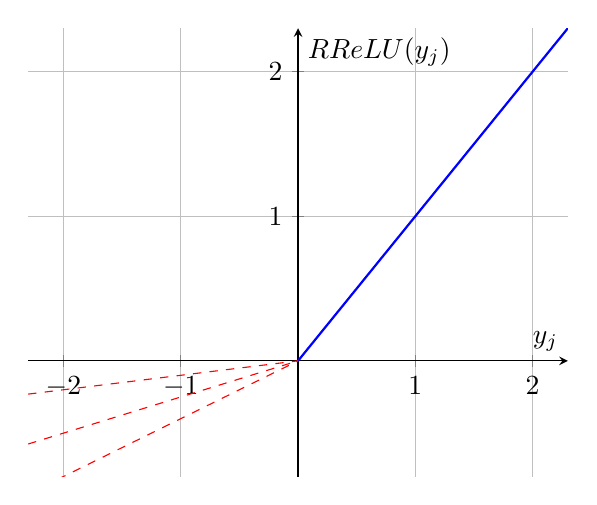
\begin{tikzpicture}
        \begin{axis}[
            xlabel={$y_j$},
            ylabel={$\text{RReLU}(y_j)$},
            xmin=-2.3, xmax=2.3,
            ymin=-0.8, ymax=2.3,
            axis lines=middle,
            grid=major,
            legend pos=north west,
            legend style={font=\tiny}
        ]
        \addplot[blue, thick, domain=0:2.3] {x};
        \addplot[red, dashed, domain=-2.3:0, samples=2] {0.1*x};
        \addplot[red, dashed, domain=-2.3:0, samples=2] {0.25*x};
        \addplot[red, dashed, domain=-2.3:0, samples=2] {0.4*x};
        \end{axis}
    \end{tikzpicture}
    \caption{Gráfico da função de ativação \textit{Randomized Leaky ReLU} (\textit{RReLU}) com diferentes inclinações aleatórias para a parte negativa.}
    \label{fig:rrelu}
    \fonte{O autor (2025).}
\end{figure}

Conhecendo como a \textit{RReLU} se comporta, é possível também calcular a sua derivada, a qual será de extrema utilidade durante a retropropagação, fazendo que os pesos e vieses do modelo sejam ajustados e com base nisso ele consiga aprender melhor o problema que está sendo analisado. Como a \textit{RReLU} utiliza a mesma fórmula que funções como a \textit{Leaky ReLU} e a \textit{PReLU}, pode-se apenas repetir a expressão de sua derivada novamente, a qual será dada pela Equação \ref{eq:rrelu-derivada}. Note que mesmo compartilhando a mesma fórmula, o termo $\alpha$ possui significado distintos em cada uma dessas funções, neste caso, ele é um valor aleatório dado pela distribuição $U(l, u)$.

Com relação ao problema da descontinuidade no ponto zero, é possível apenas escolher para qual valor essa função irá retornar neste caso, assim, vamos considerar que quando a sua entrada for zero, ela irá retornar o segundo caso, em que é a própria constante $\alpha$

\begin{equacaodestaque}{\textit{Randomized Leaky ReLU} (\textit{RReLU}) Derivada}
    \frac{d}{dy_j} [\mathcal{A}_{\text{RReLU}}](y_j) = \begin{cases}1, & \text{se } y_j > 0 \\ \alpha_i, & \text{se } y_j \leqslant  0 \end{cases}
    \label{eq:rrelu-derivada}
\end{equacaodestaque}

Esse detalhe da aleatoriedade da constante $\alpha$ afetou o desenho do gráfico da \textit{RReLU}, e com isso, ele também afeta a plotagem de sua derivada. Como pode ser visto na Figura \ref{fig:rrelu-derivada}, existem um conjunto de retas em um intervalo, neste caso, está sendo considerado a distribuição como sendo de $U(0.1, 0.3)$, mas para cada uma dessas distribuições, terá um conjunto de retas diferentes e com isso gráficos distintos para cada um dos problemas.

\begin{figure}[h!]
    \centering
    \begin{tikzpicture}
        \begin{axis}[
            xlabel={$y_j$},
            ylabel={$\text{RReLU}'(y_j)$},
            xmin=-2.3, xmax=2.3,
            ymin=-0.2, ymax=1.2,
            axis lines=middle,
            grid=major,
            legend pos=north west,
            legend style={font=\scriptsize}
        ]
        % Define l e u para a distribuição uniforme U(l,u)
        \def\lVal{0.1}
        \def\uVal{0.3}

        % Plota a derivada para z > 0
        \addplot[red, thick, domain=0:2.1] {1};
        \addlegendentry{$f'(y_j) = 1$}

        % Plota a região hachurada para z < 0
        \addplot[
            pattern=north east lines, 
            pattern color=blue!50,
            draw=none
        ] coordinates {(-2.1, \lVal) (0, \lVal) (0, \uVal) (-2.1, \uVal)} -- cycle;
        \addlegendentry{$\alpha_i \sim U(l,u)$}

        % Marcadores na descontinuidade
        \addplot[blue, only marks, mark=o, mark size=1.5pt, forget plot] coordinates {(0,\lVal)};
        \addplot[blue, only marks, mark=o, mark size=1.5pt, forget plot] coordinates {(0,\uVal)};
        \addplot[red, only marks, mark=*, mark size=1.5pt, forget plot] coordinates {(0,1)};
        
        \end{axis}
    \end{tikzpicture}
    \caption{Gráfico da derivada da função de ativação \textit{Randomized Leaky ReLU} (\textit{RReLU}) com $l=0.1, u=0.3$.}
    \label{fig:rrelu-derivada}
    \fonte{O autor (2025).}
\end{figure}

Ainda no artigo, \textcite{XuRReLU} investigam a performance de diferentes funções retificadoras em uma rede neural convolucional, cuja arquitetura pode ser vista na Tabela \ref{tab:nin_arquitetura}, para a classificação de imagens, os autores analisaram a \textit{ReLU} tradicional, a \textit{Leaky ReLU}, a \textit{Parametric ReLU} e a \textit{Randomized Leaky ReLU}. Para fazer a análise dos modelos, foram escolhidos os datasets \textit{CIFAR-10} e \textit{CIFAR-100}, e o desempenho dessas funções nos respectivos datasets pode ser visto na Tabela \ref{tab:rrelu-cifar-10} e na Tabela \ref{tab:rrelu-cifar-100}.

\begin{table}[ht]
    \centering
    \begin{threeparttable}
        \caption{Estrutura da Rede "Network in Network" (NIN) para CIFAR-10/100}
        \label{tab:nin_arquitetura}
        \begin{tabular}{ll}
            \toprule
            \textbf{Tamanho da Entrada} & \textbf{Camada / Operação} \\
            \midrule
            
            $32 \times 32$ & Conv 5x5, 192 canais \\
            $32 \times 32$ & Conv 1x1, 160 canais \\
            $32 \times 32$ & Conv 1x1, 96 canais \\
            $32 \times 32$ & Max Pooling 3x3, stride /2 \\
            \addlinespace % Adiciona espaço para separar os blocos
            
            $16 \times 16$ & Dropout, taxa 0.5 \\
            $16 \times 16$ & Conv 5x5, 192 canais \\
            $16 \times 16$ & Conv 1x1, 192 canais \\
            $16 \times 16$ & Conv 1x1, 192 canais \\
            $16 \times 16$ & Avg Pooling 3x3, stride /2 \\
            \addlinespace
            
            $8 \times 8$ & Dropout, taxa 0.5 \\
            $8 \times 8$ & Conv 3x3, 192 canais \\
            $8 \times 8$ & Conv 1x1, 192 canais \\
            $8 \times 8$ & Conv 1x1, 10 ou 100 canais\textsuperscript{a} \\
            $8 \times 8$ & Global Avg Pooling 8x8 \\
            \addlinespace
            
            10 ou 100 & Softmax \\
            
            \bottomrule
        \end{tabular}
        
        \begin{tablenotes}[para]
            \small
            \item[] Nota: Descrição da arquitetura da rede convolucional "Network in Network" (NIN). A coluna "Tamanho da Entrada" indica a dimensão espacial dos mapas de características em cada estágio. A coluna "Camada / Operação" detalha a sequência de operações da rede. \textsuperscript{a}O número de canais na última camada convolucional corresponde ao número de classes do dataset (10 para CIFAR-10 ou 100 para CIFAR-100), funcionando como uma etapa de classificação antes do Global Average Pooling.
            \item[] Fonte: Adaptado de "Empirical Evaluation of Rectified Activations in Convolutional Network", por B. Xu, N. Wang, T. Chen, \& M. Li, 2015, \textit{arXiv preprint arXiv:1505.00853}.
        \end{tablenotes}
        
    \end{threeparttable}
\end{table}

Analisando a Tabela \ref{tab:rrelu-cifar-10}, que mostra a taxa de erro das funções retificadoras na rede \textit{NIN} para o \textit{dataset CIFAR-10}, é possível notar que a \textit{Randomized Leaky ReLU} foi a função que performou melhor, com um total de 11.19\% de erro nos casos de teste, enquanto a \textit{leaky ReLU} com $a = 100$ obteve o pior resultado. Contudo, essa diferença de resultado é pequena, indicando que caso essas funções sejam muito mais complexas quando comparadas com a \textit{ReLU} na hora de treinar o modelo, pode ser melhor optar por uma função mais "barata" mas com uma taxa de erro um pouco maior.

\begin{table}[ht]
    \centering
    \begin{threeparttable}
        \caption{Taxa de Erro de Diferentes Funções de Ativação na Rede NIN para o CIFAR-10}
        \label{tab:rrelu-cifar-10}
        \begin{tabular}{lcc}
            \toprule
            \textbf{Função de Ativação} & \textbf{Erro de Treino} & \textbf{Erro de Teste (\%)} \\
            \midrule
            
            ReLU                      & 0.00318 & 12.45 \\
            \addlinespace % Adiciona um espaço para agrupar as Leaky ReLUs
            Leaky ReLU ($a=100$)      & 0.00310 & 12.66 \\
            Leaky ReLU ($a=5.5$)      & 0.00362 & 11.20 \\
            \addlinespace
            PReLU                     & 0.00178 & 11.79 \\
            \addlinespace
            RReLU\textsuperscript{a}  & 0.00550 & \textbf{11.19} \\
            
            \bottomrule
        \end{tabular}
        
        \begin{tablenotes}[para]
            \small
            \item[] Nota: Comparação da taxa de erro da rede "Network in Network" (NIN) treinada no conjunto de dados CIFAR-10 com diferentes funções de ativação retificadoras. Os valores de erro de teste são apresentados em porcentagem (\%). O valor em negrito indica o melhor resultado (menor erro de teste). \textsuperscript{a}Randomized Leaky ReLU (RReLU), onde o coeficiente de vazamento é amostrado de uma distribuição uniforme durante o treino. A fórmula na tabela original representa uma parametrização específica testada.
            \item[] Fonte: Adaptado de "Empirical Evaluation of Rectified Activations in Convolutional Network", por B. Xu, N. Wang, T. Chen, \& M. Li, 2015, \textit{arXiv preprint arXiv:1505.00853}.
        \end{tablenotes}

    \end{threeparttable}
\end{table}

Já ao analisar a Tabela \ref{tab:rrelu-cifar-100}, que mostra a taxa de erro dessas funções no \textit{dataset CIFAR-10}, é possível ver que assim como no \textit{CIFAR-10}, a \textit{RReLU} foi a função que obteve melhor resultado, neste caso há uma diferença de 2.65 pontos percentuais, quando comparada com a \textit{ReLU} tradicional. Outro ponto interessante a ser destacado ao analisar essa tabela é de que provavelmente a rede que utilizou a \textit{Parametric ReLU} sofreu um sobreajuste (\textit{overfitting}) fazendo com que ela decorasse o dados de treino e com isso conseguisse uma taxa de erro consideravelmente menor, já quando ela foi apresentada para o conjunto de testes houve uma grande disparidade das taxas de erro.

\begin{table}[ht]
    \centering
    \begin{threeparttable}
        \caption{Taxa de Erro de Funções de Ativação na Rede NIN para o CIFAR-100}
        \label{tab:rrelu-cifar-100}
        \begin{tabular}{lcc}
            \toprule
            \textbf{Função de Ativação} & \textbf{Erro de Treino (\%)} & \textbf{Erro de Teste (\%)} \\
            \midrule
            
            ReLU                      & 13.56 & 42.90 \\
            \addlinespace
            Leaky ReLU ($a=100$)      & 11.55 & 42.05 \\
            Leaky ReLU ($a=5.5$)      & 8.54  & 40.42 \\
            \addlinespace
            PReLU                     & \textbf{6.33}  & 41.63 \\
            \addlinespace
            RReLU\textsuperscript{a}  & 11.41 & \textbf{40.25} \\
            
            \bottomrule
        \end{tabular}
        
        \begin{tablenotes}[para]
            \small
            \item[] Nota: Comparação da taxa de erro (\%) da rede "Network in Network" (NIN) treinada no conjunto de dados CIFAR-100. Os valores em negrito indicam o melhor resultado (menor erro) em cada coluna. \textsuperscript{a}Randomized Leaky ReLU (RReLU), onde o coeficiente de vazamento é amostrado de uma distribuição uniforme durante o treino.
            \item[] Fonte: Adaptado de "Empirical Evaluation of Rectified Activations in Convolutional Network", por B. Xu, N. Wang, T. Chen, \& M. Li, 2015, \textit{arXiv preprint arXiv:1505.00853}.
        \end{tablenotes}
        
    \end{threeparttable}
\end{table}

Ainda em \textit{Empirical Evaluation of Rectified Activations in Convolutional Network} \textcite{XuRReLU} explicam que a \textit{RReLU} é uma função que ajuda a combater o sobreajuste (overfitting) do modelo, mas ainda devem ser feitos mais testes para descobrir como a aleatoriedade afeta os processos de treino e teste \parencite{XuRReLU}. Essa característica de ajudar a combater o sobreajuste é uma vantagem que a \textit{RReLU} possui, permitindo com que modelos maiores e mais profundos possam ser criados e mesmo assim obtenham resultados significativos. Provavelmente, um dos motivos dela possuir essa função está no fato de que ela introduz uma maior aleatoriedade para o modelo, ajudando a impedir que ele decore os padrões, como em imagens dos conjuntos \textit{CIFAR-10} e \textit{CIFAR-100}.

\medskip
\begin{center}
 * * *
\end{center}
\medskip

\textbf{Algumas Aplicações da Randomized Leaky ReLU em Redes Neurais}
\vspace{1em}

\begin{itemize}
    \item \textbf{Aplicação 1 (Área):}
    \item \textbf{Aplicação 2 (Área):}
    \item \textbf{Aplicação 3 (Área):}
    \item \textbf{Aplicação 4 (Área):}
\end{itemize}

\section{As Variantes Não Lineares: Em Busca da Suavidade}

Seguindo adiante, agora será visto um novo conjunto de variantes da \textit{ReLU} tradicional, elas incluem funções que apresentam gráficos com curvas mais suaves, como é o caso da \textit{ELU}, que faz uso de funções exponenciais para a sua composição e com isso consegue não só resolver o problema dos \textit{ReLUs} agonizantes, mas também sendo uma função contínua na origem e portanto derivável em todo o seu domínio.

Além disso, é possível conhecer também uma variante da \textit{ELU}, a \textit{Scaled Exponetial Linear Unit}, uma função que é utilizada para construir redes capazes de se autonormalizarem, ademais será visto a \textit{Noisy ReLU}, outra variante da \textit{ReLU}, mas que dessa vez adiciona ruído em sua saída a fim de garantir uma melhor performance quando comparada com a sua função original.

\subsection{Exponential Linear Unit (ELU)}

Continuando com as analogias do vendedor de pipoca, o vendedor de pipoca que faz uso da \textit{ELU} para as suas vendas trabalha de forma diferente. Ao invés de vender um punhado de pipoca de forma linear com base no dinheiro que o cliente tem quando ele não quer comprar o pacote inteiro por não possuir o valor total, ele adota uma curva exponencial como base, assim, clientes com valores muito próximos de R\$ 5,00 recebem uma quantia muito grande de pipoca, quase equivalente ao pacote total, enquanto aqueles que possuem valores pequenos irão receber um punhado pequeno de pipoca. Talvés seja uma forma de incentivar aqueles que quase tem o valor total para comprar uma pipoca, mas ainda sim garantir a clientela dos que possuem pouco dinheiro e aumentando o seu lucro como vendendor.

A \textit{ELU} ou \textit{Exponential Linear Unit} foi introduzida no artigo \textit{Fast and Accurate Deep Networks Leaning By Exponential Linear Units (ELUs)}, sendo uma variação que acelera o aprendizado de uma rede neural densa e apresentando uma maior acurácia em problemas de classificação \parencite{ELUArticle}.

A \textit{Exponential Linear Unit} pode é descrita utilizando a Equação \ref{eq:elu}. Note que há uma grande diferença dela quando comparamos com a \textit{ReLU}, a \textit{ELU} faz uso de funções exponenciais, algo que é computacionalmente mais "caro" para um computador quando comparado com apenas cálculos simples como uma função identidade.

\begin{equacaodestaque}{\textit{Exponential Linear Unit} (\textit{ELU})}
    \mathcal{A}_{\text{ELU}}(y_j) = \begin{cases}y_j, & \text{se } y_j \ge 0 \\ \alpha \cdot (e^{y_j} - 1), & \text{se } y_j < 0\end{cases}
    \label{eq:elu}
\end{equacaodestaque}

Conhecendo como é a fórmula da \textit{ELU}, é possível também plotar o seu gráfico, o qual está presente na Figura \ref{fig:elu}. Ao analisar, é possível ver uma diferença notável quando o comparada com as funções vistas anterioemente, a \textit{ELU} não apresenta um bico no ponto de origem, ela é uma função bem mais suave. Além disso, note que ela segue o mesmo padrão das outras funções: ela retorna a função identidade nos casos em que a entrada é maior que zero, assim como as outras variantes, mas quando é tratado dos casos em que a entrada é negativa, nota-se que ela utiliza uma funcão exponencial, o que garante a suavidade vista no gráfico. Perceba também que ela possui valores negativos, assim como as variantes com vazamento, indicando que ela também pode ser capaz de lidar com o problema do \textit{ReLUS} agonizantes causado pela \textit{ReLU} tradicional e que vem sendo mitigado com outras variantes como a \textit{Leaky ReLU}.

\begin{figure}[h!]
    \centering
    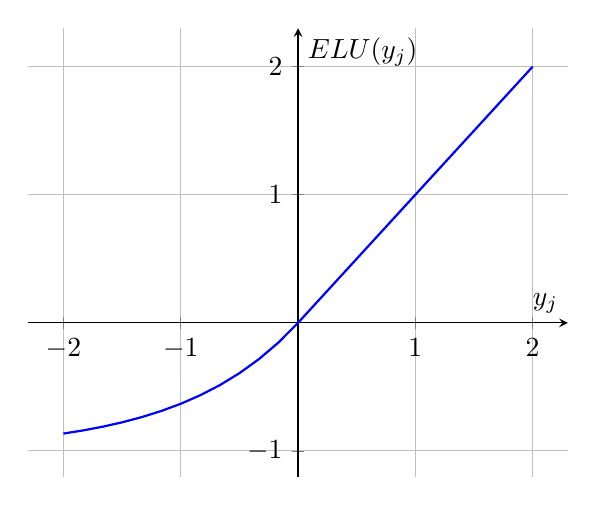
\begin{tikzpicture}
        \begin{axis}[
            xlabel={$y_j$},
            ylabel={$\text{ELU}(y_j)$},
            xmin=-2.3, xmax=2.3,
            ymin=-1.2, ymax=2.3,
            axis lines=middle,
            grid=major,
        ]
        % Define alpha para o gráfico. O valor comum para ELU é 1.
        \def\alphaVal{1} 
        \addplot[blue, thick, domain=-2:2] {x >= 0 ? x : \alphaVal*(exp(x) - 1)};
        \end{axis}
    \end{tikzpicture}
    \caption{Gráfico da função de ativação \textit{Exponential Linear Unit} (\textit{ELU}) com $\alpha=1$.}
    \label{fig:elu}
    \fonte{O autor (2025).}
\end{figure}

Agora que a sua fórmula e seu gráfico são conhecidos, cabe também calcular a sua derivada, a qual será útil na retropropagação do modelo. Para isso, é possível seguir a mesma estratégia vista até agora, derivando a função em cada um dos casos, gerando assim a sua derivada. Nos cenários em que a entrada é positiva, a derivada será sempre 1, pois quando derivamos a expressão $x$, ela nos irá retornar 1. Já quando temos o cenário negativo, teremos como resultado da derivação da expressão $alpha \cdot (e^{y_j} - 1)$ o termo $alpha \cdot e^{y_j}$. Um ponto a ser destacado é de que a \textit{ELU} é contínua na origem, assim, não tendo que preocupar em escolher um valor da derivada quando o seu valor de entrada for zero. Assim, tem-se como resultado final a Equação \ref{eq:elu-derivada}

\begin{equacaodestaque}{\textit{Exponential Linear Unit} (\textit{ELU}) Derivada}
    \frac{d}{dy_j} [\mathcal{A}_{ELU}](y_j) = \begin{cases}1, & \text{se } y_j > 0 \\ \alpha \cdot e^{y_j}, & \text{se } y_j \le 0 \end{cases}
    \label{eq:elu-derivada}
\end{equacaodestaque}

Sabendo a sua derivada, pode-se também plotar o seu gráfico, para isso, ele está representado na Figura \ref{fig:elu-derivada}. Note que ele é composto de duas partes diferentes, sendo a primeira delas, para os casos em que a entrada é negativa, a função constante em um, e para os casos em que a entrada é negativa, tem-se uma curva exponencial. Perceba também que a sua derivada irá sempre retornar valores positivos quando é calculada para qualquer ponto do seu domínio.

\begin{figure}[h!]
    \centering
    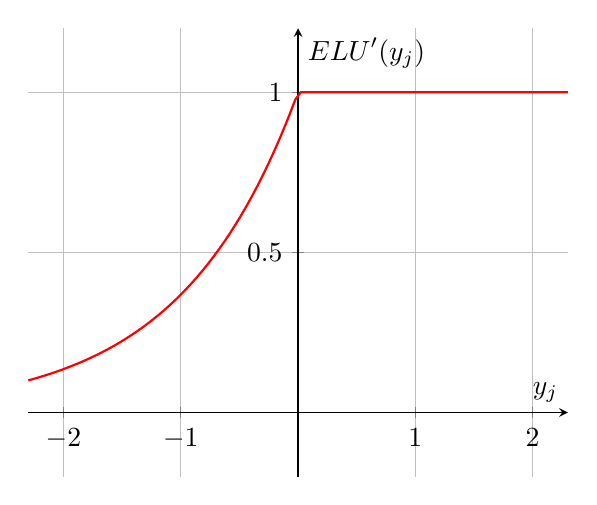
\begin{tikzpicture}
        \begin{axis}[
            xlabel={$y_j$},
            ylabel={$\text{ELU}'(y_j)$},
            xmin=-2.3, xmax=2.3,
            ymin=-0.2, ymax=1.2,
            axis lines=middle,
            grid=major
        ]
        % Define alpha para o gráfico
        \def\alphaVal{1} 

        % Plota a derivada usando uma única expressão condicional
        \addplot[red, thick, domain=-2.3:2.3, samples=100] {x > 0 ? 1 : \alphaVal*exp(x)};
        
        \end{axis}
    \end{tikzpicture}
    \caption{Gráfico da derivada da função de ativação \textit{Exponential Linear Unit} (\textit{ELU}) com $\alpha=1$.}
    \label{fig:elu-derivada}
    \fonte{O autor (2025).}
\end{figure}

Um dos testes realizados pelos autores para analisar o desempenho na \textit{ELU}, foi na criação de uma \textit{CNN} com 18 camadas convolucionais para fazer a classifição dos datasets \textit{CIFAR-10} e \textit{CIFAR-100}, para isso, outras técnicas foram utilizas em conjunto como o decaimento do peso L2 e reduções das taxas de aprendizado \parencite{ELUArticle}.

Com base nessa \textit{CNN} e seus experimentos, é possível ver os resultados na Tabela \ref{tab:elu-cifar-comparativo}, em que \textcite{ELUArticle} comparam a \textit{ELU} com outras redes no mesmo problema, como a \textit{AlexNet} que foi vista anterioremente na explicação do surgimento da \textit{ReLU}. Ao analisar esses resultados, nota-se que a \textit{ELU} obteve um desempenho excelente no dataset \textit{CIFAR-100}, com uma diferença de 21.52 pontos percentuais quando comparada com a \textit{AlexNet}, que ficou em último lugar. Já ao considerar o seu desempenho para um problema de classificação mais simples, como o \textit{CIFAR-10}, ela ficou em segundo lugar, estando atrás apenas da \textit{Fract. Max-Pooling}, mas ainda sim, apresentando uma diferença considerável de 2.05 pontos percentuais a mais de erro. 

\begin{table}[ht]
    \centering
    \begin{threeparttable}
        \caption{Comparativo da Taxa de Erro de Redes Neurais nos Datasets CIFAR}
        \label{tab:elu-cifar-comparativo}
        \begin{tabular}{lccc}
            \toprule
            \textbf{Arquitetura da Rede} & \textbf{CIFAR-10 Erro (\%)} & \textbf{CIFAR-100 Erro (\%)} & \textbf{Augmentation} \\
            \midrule
            
            AlexNet              & 18.04          & 45.80          &                \\ 
            \addlinespace
            DSN                  & 7.97           & 34.57          & v              \\
            NiN                  & 8.81           & 35.68          & v              \\
            Maxout               & 9.38           & 38.57          & v              \\
            All-CNN              & 7.25           & 33.71          & v              \\
            Highway Network      & 7.60           & 32.24          & v              \\
            Fract. Max-Pooling   & \textbf{4.50}  & 27.62          & v              \\
            ELU-Network          & 6.55           & \textbf{24.28} & v              \\
            
            \bottomrule
        \end{tabular}
        
        \begin{tablenotes}[para]
            \small
            \item[] Nota: Comparação da taxa de erro de classificação (\%) no conjunto de teste para diversas arquiteturas de redes neurais convolucionais (CNNs). Os valores em negrito indicam o melhor resultado em cada dataset. A coluna "Augmentation" indica se foram utilizadas técnicas de aumento de dados (data augmentation) durante o treinamento, marcado com "v".
            \item[] Fonte: Adaptado de "Fast and Accurate Deep Network Learning by Exponential Linear Units (ELUs)", por D. Clevert, T. Unterthiner, \& S. Hochreiter, 2015, \textit{arXiv preprint arXiv:1511.07289}.
        \end{tablenotes}
        
    \end{threeparttable}
\end{table}

Isso indica que a \textit{ELU} é uma excelente opção para problemas de classificação, especialmente se há um grande número de classes a ser analisadas. Contudo, uma rede neural convolucional que apresenta 18 camadas de convolução pode ser um tanto quanto custosa para ser processada por um computador, assim, faz se necessário o uso de unidades de \textit{GPUs} para o processamento de uma rede como essa, para que mesmo sendo pesada para ser processada, os resultados possam sair um pouco mais rápidos.

Por fim, cabe destacar algumas afirmações realizadas pelos autores ainda em \textit{Fast and Accurate Deep Networks Leaning By Exponential Linear Units (ELUs)}, segundo \textcite{ELUArticle}, ao comparar a \textit{ELU} com funções como a \textit{ReLU tradicional} e \textit{Leaky ReLU}, pode-se notar um melhor e mais rápido aprendizado, além de que a \textit{Exponetial Linear Unit} é capaz de garantir uma melhor generalização quando passa a ser utilizada em redes com mais de cinco camadas. Outro ponto destacado pelos autores, está no fato da \textit{ELU} garantir \textit{noise rebust deactivation states}, algo que mesmo com a \textit{Leaky ReLU} e \textit{Parametric ReLU} possuindo valores negativos, não são capazes de garantir ao serem utilizadas para construir uma rede neura \parencite{ELUArticle}.

Mesmo apresentando um grande salto, quando comparada com a \textit{ReLU} tradicional, a \textit{ELU} também pode ser modificada para atender outros casos. Para isso, ela também tem variações, sendo uma delas a \textit{SELU}, a qual adiciona a \textit{ELU} um termo $\lambda$ para garantir uma autonormalização da rede que está sendo criada. Essa função será vista em seguida.

\medskip
\begin{center}
 * * *
\end{center}
\medskip

\textbf{Algumas Aplicações da Exponential Linear Unit em Redes Neurais}
\vspace{1em}

\begin{itemize}
    \item \textbf{Aplicação 1 (Área):}
    \item \textbf{Aplicação 2 (Área):}
    \item \textbf{Aplicação 3 (Área):}
    \item \textbf{Aplicação 4 (Área):}
\end{itemize}

\subsection{Scaled Exponential Linear Unit (SELU)}

A próxima função é uma variante da \textit{ELU}, a \textit{Scaled Exponential Linear Unit}, ou \textit{SELU}. Ela se distingue da ELU tradicional pelo fato de que ela é capaz de implemtar propriedades auto-normalizadoras em uma rede que faz uso dessa função, como explicam os autores no artigo de sua introdução \textit{Self-Normalizing Neural Networks} \parencite{SELUArticle}.

Os autores apresentam a Equação \ref{eq:selu} para calcular essa função, em que o termo $\lambda$ é uma constante que será maior que 1 \parencite{SELUArticle}. Note que essa fórmula é bem parecida com a da \textit{Exponential Linear Unit}, a única diferença é que ela estará sendo multiplicada pela constante $\lambda$, assim pode-se escrever também que $\text{SELU}(y_j) = \lambda \text{ELU}(y_j)$.

\begin{equacaodestaque}{\textit{Scaled Exponential Linear Unit} (\textit{SELU})}
    \mathcal{A}_{\text{SELU}}(y_j) = \lambda \begin{cases}y_j, & \text{se } y_j > 0 \\ \alpha \cdot (e^{y_j} - 1), & \text{se } y_j \le 0\end{cases} \quad \text{ou} \quad \mathcal{A}_{\text{SELU}}(y_j) = \lambda \text{ELU}(y_j)
    \label{eq:selu}
\end{equacaodestaque}

Com relação ao seu gráfico, ele está presente na Figura \ref{fig:selu}, neste caso, está sendo considerado que as constantes $\alpha$ e $\lambda$ são dadas por 1.7 e 1.05 respectivamente. Note que é um gráfico que lembra bastante a \textit{Leaky ReLU}, mas que neste caso, quando a função recebe valores negativos, ela não estará mais assumindo o comportamento de uma reta, e sim o de uma curva exponencial, já para os cenários em que a entrada é postiva os resultados serão próximos os de uma função identidade, mas com uma reta um pouco mais inclinada. 

Pelo fato da \textit{SELU} ter um comportamento que também retorna valores para a saída quando a sua entrada é negativa, ela consegue combater o problema dos \textit{ReLUs} agonizantes, causado pela \textit{ReLU}, além de que também não é uma função saturante, como a sigmoide, o que também ajuda a resolver o problema no desaparecimento do gradiente. Mas, por não ser uma função saturante, e pelo fato de que sua saída vai para valores infinitos conforme os valores de sua entrada aumentam, ela está sujeita ao problema da explosão de gradientes.

\begin{figure}[h!]
    \centering
    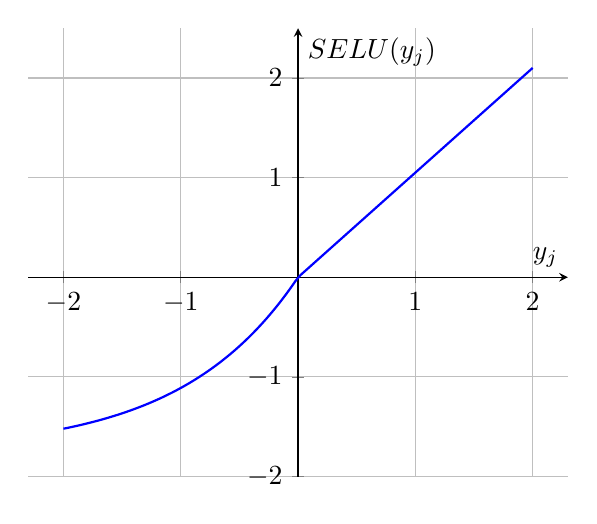
\begin{tikzpicture}
        \begin{axis}[
            xlabel={$y_j$},
            ylabel={$\text{SELU}(y_j)$},
            xmin=-2.3, xmax=2.3,
            ymin=-2, ymax=2.5,
            axis lines=middle,
            grid=major,
        ]
        % Define as constantes da SELU para o gráfico
        \def\alphaVal{1.67326}
        \def\lambdaVal{1.0507}
        \addplot[blue, thick, domain=-2:2, samples=100] {x > 0 ? \lambdaVal*x : \lambdaVal*\alphaVal*(exp(x) - 1)};
        \end{axis}
    \end{tikzpicture}
    \caption{Gráfico da função de ativação \textit{Scaled Exponential Linear Unit} (\textit{SELU}) com $\alpha \approx 1.67 e \lambda \approx 1.05$.}
    \label{fig:selu}
    \fonte{O autor (2025).}
\end{figure}

Considerando agora como é a equação da \textit{SELU} e qual é o seu comportamento no gráfico, é possível também calcular a sua derivada para ser utilizada na retroproapagação do gradiente, para isso, deve-se derivar a Equação \ref{eq:selu}, considerando os dois cenários, em que a sua entrada será positiva e quando sua entrada for negativa ou zero. Um ponto que ajuda bastante ao calcular a derivada da \textit{SELU} está no fato dela ser composta pela função \textit{ELU} multiplicada por uma constante, se utilizarmos regras de derivação para esse cenário, precisaremos apenas derivar a \textit{ELU} e depois adicionar a constante $\lambda$ multiplicando-a. Como a derivada da \textit{ELU} já foi calculada, ela pode ser aproveitada agora. Você pode ver então a derivada da \textit{Scaled Exponential Linear Unit} na Equação \ref{eq:selu-derivada}.

\begin{equacaodestaque}{\textit{Scaled Exponential Linear Unit} (\textit{SELU}) Derivada}
    \frac{d}{dy_j} [\mathcal{A}_{SELU}](y_j) = \lambda \begin{cases}1, & \text{se } y_j > 0 \\ \alpha \cdot e^{y_j}, & \text{se } y_j \le 0\end{cases}
    \label{eq:selu-derivada}
\end{equacaodestaque}

Sabendo a sua derivada, é possível também plotar o seu gráfico, para isso, ele está na Figura \ref{fig:selu-derivada}. Note, que o gráfico da derivada da \textit{SELU} também possui grandes similaridades com a \textit{ELU} original mas também com as outras retificadoras, pois também pode ser dividido em duas partes principais. A primeira parte, para os casos em que a entrada é negativa segue o comportamento de uma curva exponencial, enquanto a segunda parte é semelhante a uma reta constante com inclinação zero. 

Um ponto interessante dessa reta da segunda parte é que ela retorna justamente um valor bem próximo de um, assim como nas retificadoras, isso trás como benefício uma menor chance para ocorrer casos de desaparecimento do gradiente, pois ele não estará sendo constantemente sendo multiplicado por valores pequenos e com isso reduzindo o seu valor. Mas, por outro lado, isso também acaba colaborando para que gradientes explosivos possam ocorrer.

\begin{figure}[h!]
    \centering
    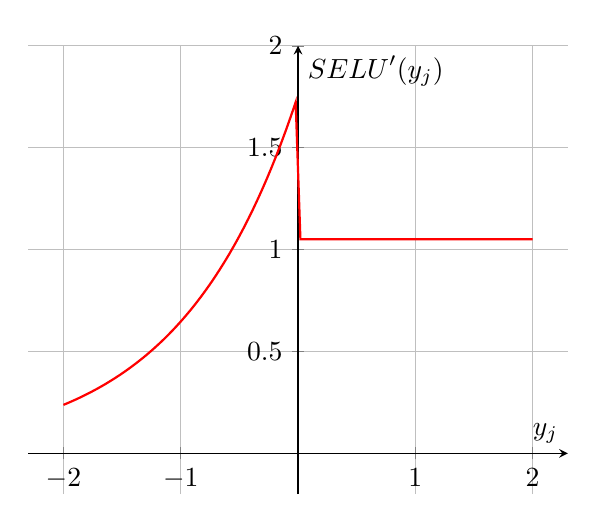
\begin{tikzpicture}
        \begin{axis}[
            xlabel={$y_j$},
            ylabel={$\text{SELU}'(y_j)$},
            xmin=-2.3, xmax=2.3,
            ymin=-0.2, ymax=2.0, % Ajustado para lambda > 1
            axis lines=middle,
            grid=major
        ]
        % Define as constantes da SELU para o gráfico
        \def\alphaVal{1.67326}
        \def\lambdaVal{1.0507}

        \addplot[red, thick, domain=-2:2, samples=100] {x > 0 ? \lambdaVal*1 : \lambdaVal*\alphaVal*exp(x)};
        \end{axis}
    \end{tikzpicture}
    \caption{Gráfico da derivada da função de ativação Scaled Exponential Linear Unit (SELU) com $\alpha \approx 1.67, \lambda \approx 1.05$.}
    \label{fig:selu-derivada}
    \fonte{O autor (2025).}
\end{figure}

No texto da introdução da \textit{SELU}, \textcite{SELUArticle}, comparam as redes neurais criadas por eles, as quais são chamadas de \textit{Self-Normalizing Neural Networks} (\textit{SNN}), com outras redes \textit{feedforward}, como \textit{MSRAinit} (uma \textit{FNN} que não possui técnicas de normalização, com funções de ativação \textit{ReLU}, e que faz uso do \textit{Microsoft weight initialization}), a \textit{BatchNorm} (uma \textit{FNN} com normalização em lote), a \textit{LayerNorm} (uma \textit{FNN} com normalização nas camadas), a \textit{WightNorm} (uma \textit{FNN} com normalização nos pesos), a \textit{Highway} e também com redes residuais \textit{ResNet}. Para comparar essas redes, os autores escolhem 121 \textit{datasets} do \textit{UCI}, em que são apresentadas áreas de aplicação diversas como física e biologia, nesses \textit{datasets} o seus tamanhos podem variar de 10 até 130.000 pontos de dados com o número de features variando de 4 a 250. Na Tabela \ref{tab:comparativo-selu}, é possível ver o ranking médio entre as \textit{SNNs} e as outras diferentes arquiteturas em 75 tarefas de classificação.

\begin{table}[ht]
    \centering
    \begin{threeparttable}
        \caption{Comparativo do Rank Médio entre SNNs e Outras Arquiteturas de Redes Neurais}
        \label{tab:comparativo-selu}
        \begin{tabular}{llcc}
            \toprule
            \textbf{Grupo do Método} & \textbf{Método} & \textbf{Rank Médio} & \textbf{Valor-p} \\
            \midrule
            
            SNN & SNN & 9.6 & $3.8 \times 10^{-1}$ \\
            MSRAinit & MSRAinit & 11.0 & $4.0 \times 10^{-2}$ \\
            LayerNorm & LayerNorm & 11.3 & $7.2 \times 10^{-2}$ \\
            Highway & Highway & 11.5 & $8.9 \times 10^{-3}$ \\
            ResNet & ResNet & 12.3 & $3.5 \times 10^{-3}$ \\
            BatchNorm & BatchNorm & 12.6 & $4.9 \times 10^{-4}$ \\
            WeightNorm & WeightNorm & 13.0 & $8.3 \times 10^{-5}$ \\

            \bottomrule
        \end{tabular}
        
        \begin{tablenotes}[para]
            \small
            \item[] Nota: Comparação do rank médio de diferentes arquiteturas de redes neurais em 75 tarefas de classificação do repositório UCI. O "Rank Médio" é a média das classificações de acurácia entre as tarefas. O "Valor-p" corresponde ao teste de Wilcoxon pareado para avaliar se a diferença para o método de melhor desempenho é significativa.
            \item[] Fonte: Adaptado de "Self-Normalizing Neural Networks", por G. Klambauer, T. Unterthiner, A. Mayr, \& S. Hochreiter, 2017, \textit{arXiv preprint arXiv:1706.02515}.
        \end{tablenotes}
        
    \end{threeparttable}
\end{table}

Para analisar essa tabela, pode-se primeiro olhar o ranking médio de cada uma desses modelos, que é dado pela média de como esses modelos performaram nos diferentes datasets, considerando isso, note que as redes que fazem uso da \textit{SELU} em sua composição, as \textit{SNNs}, são as melhores, por uma diferença de 1.4 pontos quando comparadas com o segundo colocado, isso indica que a \textit{SELU} pode ser uma ótima alternativa quando ainda não se sabe exatamente qual será o conjunto de dados que será trabalhado, se ele será de conceitos como física ou geologia, assim, elas garantem uma maior versatilidade para encarar diversos problemas. Além disso, ao olhar também o seu \textit{p-value}, que vem de um teste de Wilcoxon pareado para verificar se a diferença em relação ao melhor colocado é signifitiva, percebe-se que as \textit{SNNs} continuam se destacando, com o \textit{p-value} mais alto, indicando que existe uma diferença que não é estatisticamente significativa quando ela é comparada com o modelo \textit{SVM}, mostrando que podemos considerar as \textit{SNNs} como se tivessem empatadas com o campeão.

O interessante dessa comparação é analisar ela considerando aquelas redes que fazem uso de técnicas de normalização para conseguir uma maior desempenho, como a \textit{BatchNorm} e a \textit{LayerNorm}, cada uma delas utiliza uma técnica de normalização diferente de forma a garantir que que problemas como os gradientes explosivos e desaparacimento do gradiente não ocorra com tanta frequência e com isso permitindo um melhor convergência do modelo que está sendo treinado. Ao olhar por essa ótica, pode-se chegar a conclusão que criar uma rede neural utilizando a \textit{SELU} não só irá garantir uma maior versatilidade para a resolução de problemas, como também você não terá que se preocupar em aplicar técnicas de normalização ao construir essa rede.

Voltando para o seu texto de introdução, os autores destacam propriedades importantes dessa nova função de atiavção criada, como o fato de que de que elas possbilitam a criação de redes neurais mais profundas além de serem capazes de aplicar fortes esquemas de regularização \parencite{SELUArticle}. Por favorecer a criação de RNAs mais profundas, como consequência, a \textit{SELU} se torna uma excelente alternativa para ser utilizada em problemas complexos, que possuem muitas características e por essa razação necessitam de que mais camadas sejam construídas a fim de garantir um melhor processamento e aprendizado dos dados e com base nisso, alcançar métricas maiores, como uma maior acurácia indicando uma gerenalização maior e também uma perda menor, indicando que o gradiente conseguiu uma convergência melhor.

\medskip
\begin{center}
 * * *
\end{center}
\medskip

\textbf{Algumas Aplicações da Scaled Exponential Linerar Unit em Redes Neurais}
\vspace{1em}

\begin{itemize}
    \item \textbf{Aplicação 1 (Área):}
    \item \textbf{Aplicação 2 (Área):}
    \item \textbf{Aplicação 3 (Área):}
    \item \textbf{Aplicação 4 (Área):}
\end{itemize}

\subsection{Noisy ReLU (NReLU)}

Seguindo adiante, é possível conhecer a \textit{Noisy ReLU}, também conhecida como \textit{NReLU}. Um dos trabalhos que explora as característica dessa função e como ela pode ser aplicada em uma RNA é o \textit{Rectified Linear Units Improve Restricted Boltzmann Machines} dos autores \textcite{Nair2010}. Nesse texto, os autores comparam o desenpenho dessa função com a função binária, dada pela equação \ref{eq:equacao-binary}, que era a opção mais comum para ser utilizada na construção de máquinas restritas de Boltzmann.

\begin{equacaodestaque}{Função de Ativação Binária (\textit{Binary})}
    \mathcal{A}(y_j) = \begin{cases} 
    1 & \text{se } y_j \ge \theta \\ 
    0 & \text{se } y_j < \theta 
    \end{cases}
    \label{eq:equacao-binary}
\end{equacaodestaque}

No texto, \textcite{Nair2010}, apresentam a \textit{NReLU} como sendo dada pela equação $\max{0, y_j + \mathcal{N}(0, \sigma(y_j))}$, em que $\mathcal{N}(0, V)$ representa o ruído Gaussiano (\textit{Gaussian noise} em inglês), com méida zero e vairância dada por $V$. Também é possível expressar a \textit{Noisy ReLU} com a Equação \ref{eq:nrelu}.

\begin{equacaodestaque}{\textit{Noisy ReLU} (\textit{NReLU})}
    \mathcal{A}_{\text{NReLU}}(y_j) = \begin{cases} 
    y_j + \mathcal{N} (0, \sigma(y_j)) & \text{se } y_j > 0 \\
    0 & \text{se } y_j \le 0
    \end{cases}
    \label{eq:nrelu}
\end{equacaodestaque}

Antes de seguir em frente, é útil entende primeiro o que é ruído gaussiano, e para isso, é preciso entender antes a distribuição gaussiana. Segundo \textcite{DeepLearningBook}, a distribuição gaussiana é a distribuição mais utilizada para números reais, ela também é conhecida por ser chamada de distribuição normal, ela é dada pela Equação \ref{eq:distribuicao-gaussiana}.

\begin{equation}
    \mathcal{N}(x; \mu, \sigma^2) = \sqrt{\frac{1}{2\pi\sigma^2}} \exp\left( -\frac{1}{2\sigma^2}(x - \mu)^2 \right)
    \label{eq:distribuicao-gaussiana}
\end{equation}

Nessa equação, os dois parâmetros $\mu \in \mathbb{R}$ e $\sigma (0, \infty)$ controlam como a distribuição normal funciona; o termo $\mu$ é responsável por dar as coordenadas para o pico do centro, que é também a média da distribuição $\mathbb{E}[x] = \mu$, já o desvio padrão é dado por $\sigma$, equanto a variância é denotada por $\sigma^2$ \parencite{DeepLearningBook}. Para chegarmos no ruído gaussiano, é preciso então adicionar como parâmetros da equação da distribução gaussiana (Equação \ref{eq:distribuicao-gaussiana}) os termos que são dados pela Equação \ref{eq:nrelu}. 

A distribuição normal, com os parâmetros $\mu = 0$ e $\sigma=1$, é responsável por gerar um gráfico em formato de sino, como é mostrado na Figura \ref{fig:distribuicao-normal-padrao}. Esse gráfico indica quais são os casos que possuem uma maior probabilidade de acontecer, os casos que estão no centro, onde, $p(x)$ possuem uma maior probabilidade de acontecer, já conforme eles se distânciam desse centro essa propabilidade diminui.

\begin{figure}[htbp]
    \centering
    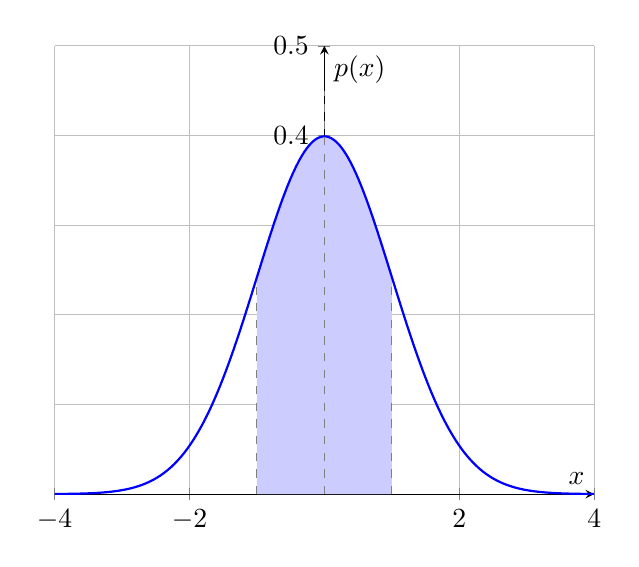
\begin{tikzpicture}
        \begin{axis}[
            xlabel={$x$},
            ylabel={$p(x)$}, % p(x) é a densidade de probabilidade
            xmin=-4, xmax=4,
            ymin=0, ymax=0.5,
            axis lines=middle,
            grid=major,
            samples=200, % Aumenta o número de pontos para uma curva mais suave
            domain=-4:4,
        ]
        
        % Declara a função da distribuição normal para facilitar o uso
        \def\normaldist#1#2{1/(#2*sqrt(2*pi))*exp(-((x-#1)^2)/(2*#2^2))}
        
        % Adiciona a área sombreada para +/- 1 desvio padrão
        \addplot[fill=blue!20, draw=none, domain=-1:1] {\normaldist{0}{1}} \closedcycle;

        % Plota a curva da distribuição normal padrão (mu=0, sigma=1)
        \addplot[blue, thick] {\normaldist{0}{1}};

        % Adiciona linhas verticais para marcar a média e os desvios padrão
        \draw[dashed, gray] (axis cs:0, 0) -- (axis cs:0, 0.45);
        \draw[dashed, gray] (axis cs:1, 0) -- (axis cs:1, 0.24);
        \draw[dashed, gray] (axis cs:-1, 0) -- (axis cs:-1, 0.24);

        % Adiciona os labels para a média e desvio padrão
        \node[below] at (axis cs:0, 0) {$\mu=0$};
        \node[below] at (axis cs:1, 0) {$\sigma$};
        \node[below] at (axis cs:-1, 0) {$-\sigma$};
        
        \end{axis}
    \end{tikzpicture}
    \caption{Gráfico da Distribuição Gaussiana (ou Normal) para o caso padrão, com média 0 ($\mu = 0$) e desvio padrão 1 ($\sigma = 1$).}
    \label{fig:distribuicao-normal-padrao}
    \fonte{O autor (2025).}
\end{figure}

Entendendo a estrutura e como funciona a \textit{Noisy ReLU}, é possível plotar o seu gráfico, o qual é dado pela Figura \ref{fig:nrelu}. Note que ela compartilha a suavidade das funções \textit{ELU} e \textit{SELU}, apresentando uma curva para os casos em que a entrada é negativa, o que é bom, pois ela permite um vazamento de gradiente, evitando assim o o problema do \textit{ReLUs} agonizantes. Já para os cenários que a entrada é positiva ela assume o comportamento de uma função identidade, lembrando bastante as outras variantes da \textit{ReLU}. Contudo, como os autores destacam no texto, ela não é capaz de resolver o problema da descontinuidade em zero, para isso, em sua derivada que é utilizada na retropropagação, os casos em que sua entrada é zero irão retornar zero como saída \parencite{Nair2010}.

\begin{figure}[h!]
    \centering
    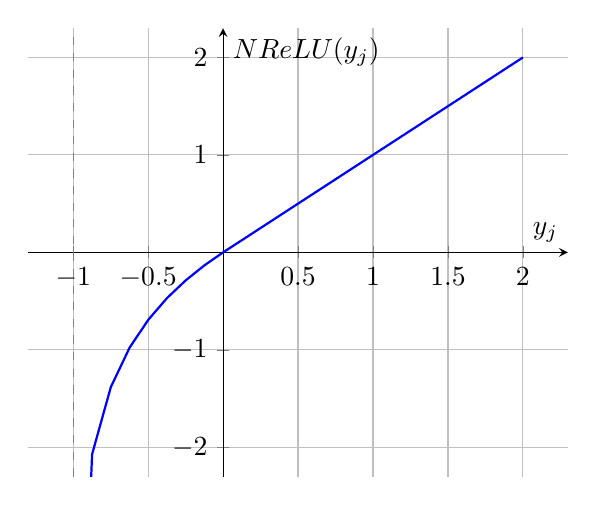
\begin{tikzpicture}
        \begin{axis}[
            xlabel={$y_j$},
            ylabel={$\text{NReLU}(y_j)$},
            xmin=-1.3, xmax=2.3,
            ymin=-2.3, ymax=2.3,
            axis lines=middle,
            grid=major,
            domain=-0.999:2, % Domínio para evitar o log de zero ou negativo
        ]
        % A função ln(1+x) está definida para x > -1
        \addplot[blue, thick] {x >= 0 ? x : ln(1+x)};
        % Linha vertical para mostrar a assíntota em z = -1
        \draw[dashed, gray] (axis cs:-1, -2.3) -- (axis cs:-1, 2.3);
        \end{axis}
    \end{tikzpicture}
    \caption{Gráfico da função de ativação \textit{Noisy ReLU} (\textit{NReLU}).}
    \label{fig:nrelu}
    \fonte{O autor (2025).}
\end{figure}

Ao calcular a derivada da \textit{NReLU} você encontrará um problema que não havia aparecido nas outras funções. O termo de ruído $\mathcal{N}$ é um termo não determísitico, o que significa que mesmo que tivéssemos a mesma entrada para a função \textit{Noisy ReLU} duas ou mais vezes, não poderíamos afirmar com certeza de que essas saídas seriam iguais. Para resolver esses problemas, os autores consideram para a \textit{NReLU} que sua função para o \textit{backward pass} será irá retornar zero quando o valor de entrada for negativo ou nulo, e irá retornar um, quando o valor de entrada for positivo \parencite{Nair2010}. Então a expressão que representa a \textit{NReLU} para a retropropagação é dada pela Equação \ref{eq:nrelu-derivada}, note que ela é a mesma expressão da derivada da \textit{ReLU} tradicional.

\begin{equacaodestaque}{\textit{Noisy ReLU} (\textit{NReLU}) para o \textit{Backward Pass}}
    \frac{d}{dy_j}{\mathcal{A}_{\text{NReLU}}}(y_j) = \begin{cases} 
        1 & \text{se } y_j > 0 \\
        0 & \text{se } y_j \le 0
    \end{cases}
    \label{eq:nrelu-derivada}
\end{equacaodestaque}

Se a função da \textit{Noisy ReLU} no \textit{backward pass} será a mesma que a derivada da \textit{ReLU}, então é possível utilizar como base o gráfico da derivada da \textit{ReLU}. Para isso, tem-se então a Figura \ref{fig:nrelu-derivada}.

\begin{figure}[htbp] % Use [htbp] para dar flexibilidade ao LaTeX
    \centering % Centraliza o gráfico na página
    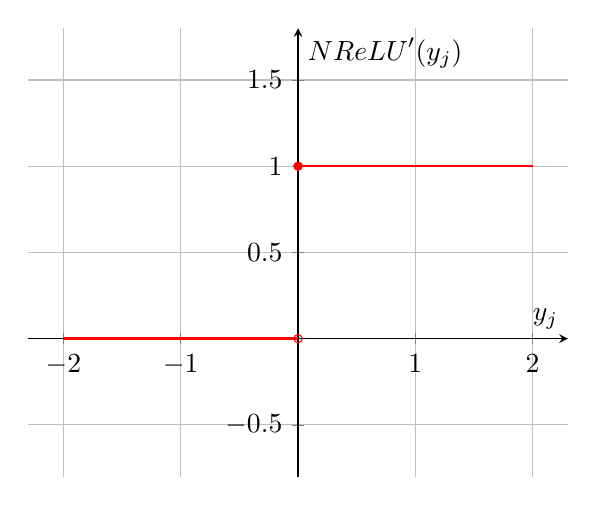
\begin{tikzpicture}
        \begin{axis}[
            xlabel={$y_j$},
            ylabel={$\text{NReLU}'(y_j)$},
            xmin=-2.3, xmax=2.3,
            ymin=-0.8, ymax=1.8,
            axis lines=middle,
            grid=major
        ]
        \addplot[red, thick, domain=-2:0] {0};
        \addplot[red, thick, domain=0:2] {1};
        \addplot[red, only marks, mark=o, mark size=1.5pt] coordinates {(0,0)};
        \addplot[red, only marks, mark=*, mark size=1.5pt] coordinates {(0,1)};
        \end{axis}
    \end{tikzpicture}
    \caption{Gráfico da função \textit{Backward Pass} da função de ativação \textit{Noisy ReLU}.}
    \label{fig:nrelu-derivada}
    \fonte{O autor (2025).}
\end{figure}

No trabalho \textit{Rectified Linear Units Improve Restricted Boltzmann Machines}, \textcite{Nair2010} exploram o desempenho da \textit{NReLU} e \textit{ReLU} utilizando o \textit{dataset NORB}, que é um \textit{dataset} para o reconhecimento de objetos 3D sintéticos que contém cinco classes: humanos, animais, carros, aviões e caminhões. No texto, os autores utilizam a versão \textit{Jittered-Cluttered NORB}, uma variante que tem imagens estereoscópicas em tons de cinza com fundo desorganizado e um objeto central que é aleatoriamente instável em posição, tamanho, intensidade de pixels \parencite{Nair2010}. O desempenho dessas funções nesse \textit{dataset} pode ser visto pela Tabela \ref{tab:norb-error-rate} e pela Tabela \ref{tab:nrelu-norb-comparativo}.

A Tabela \ref{tab:norb-error-rate}, mostra a taxa de erro dos diferentes modelos no \textit{dataset}, para isso, são construídos modelos com 4000 unidades ocultas treinados com imagens de dimensões 32x32x2. Note ao analisar a tabela que é nítido que os modelos que são pré-treinados utilizando máquinas de Boltzmann restritas apresentam um melhor desempenho de forma geral, da mesma forma que a \textit{NReLU} oferece uma perda menor quando comparada com a função binária em ambos os casos: pré-treinado ou não. 

Mas, vale a pena fazer uma comparação ainda mais interessante, o modelo que faz uso da \textit{Noisy ReLU} que não foi pré-treinado apresenta um resultado com uma diferença de 0.9 pontos quando comparado com o modelo treinado que faz uso da função binária. Isso é interessante porque indica que é possível conseguir um resultado muito melhor utilizando a \textit{Noisy ReLU} mediante a função binária mesmo quando não tiver condições de pré-treinar uma rede.

\begin{table}[ht]
    \centering
    \begin{threeparttable}
        \caption{Taxa de Erro de Classificadores no Dataset NORB Jittered-Cluttered}
        \label{tab:norb-error-rate}
        \begin{tabular}{lcc}
            \toprule
            \textbf{Pré-treinado?} & \textbf{NReLU (\%)} & \textbf{Binary (\%)} \\
            \midrule
            
            Não & 17.8 & 23.0 \\
            Sim & \textbf{16.5} & \textbf{18.7} \\
            
            \bottomrule
        \end{tabular}
        
        \begin{tablenotes}[para]
            \small
            \item[] Nota: Taxas de erro no conjunto de teste para classificadores com 4000 unidades ocultas. Os valores em negrito indicam a menor taxa de erro (melhor resultado) em cada coluna. Os modelos foram treinados com imagens de 32x32x2 do dataset NORB Jittered-Cluttered. A coluna "NReLU" refere-se a unidades de ativação ReLU com ruído (Noisy ReLU), enquanto "Binary" refere-se a unidades binárias tradicionais. A coluna "Pré-treinado?" indica se o modelo utilizou uma Máquina de Boltzmann Restrita para pré-treinamento.
            \item[] Fonte: Adaptado de "Rectified Linear Units Improve Restricted Boltzmann Machines", por V. Nair \& G. E. Hinton, 2010, \textit{Proceedings of the 27th International Conference on Machine Learning (ICML-10)}.
        \end{tablenotes}
        
    \end{threeparttable}
\end{table}

Seguindo adiante, na Tabela \ref{tab:nrelu-norb-comparativo} também é possível analisar as taxas de erro dos classicadores, mas, neste caso, eles possuem duas camadas ao invés de somente uma como mostrado da comparação da Tabela \ref{tab:norb-error-rate}, assim a primeira camada é composta de 4000 unidades ocultas (assim como no primeiro caso), enquanto a segunda camada possui 2000 unidades ocultas. 

Com base essa tabela, é possível notar que o desempenho dos modelos que fazem uso da \textit{Noisy ReLU} melhorou tanto nos casos em que as camadas não foram pré-treinadas, quanto nos casos em que uma ou ambas foram, quando se compara com os resultados da Tabela \ref{tab:norb-error-rate}. Um ponto interessante disso é que no caso em que somente uma das camadas foi pré-treinada no modelo que usa a \textit{NReLU} o seu resultado foi igual ao do primeiro caso onde existia somente uma camada, o que pode indicar que talvez não seja vantajoso adicionar mais camadas em uma rede caso não esteja disposto a pré-treiná-las. Note também que esse cenário com a unidade binária foi ainda pior, mostrando que não existe um grande ganho em adicionar mais camadas em uma rede que faz uso dessa função.

Esse resultado prová-se ainda mais nítido quando é analisado o caso em que ambas as camadas foram pré-treinadas, na unidade binária não houve nenhuma diminuição na sua perda, ela inclusive é pior que a do modelo que faz uso de apenas uma camada. Já quando é observada a \textit{Noisy ReLU} e seus resultados, nota-se um cenário bem diferente, os modelos que fazem uso dela apresentam um desempenho melhor quando são adicionadas mais camadas na rede, fazendo com que a perda da rede diminua, indicando que essa função permite a criação de redes mais profundas e com isso, desempenhos melhores possam ser alcançados.

\begin{table}[ht]
    \centering
    \begin{threeparttable}
        \caption{Taxas de Erro de Classificadores no Dataset Jittered-Cluttered NORB}
        \label{tab:nrelu-norb-comparativo}
        \begin{tabular}{llcc}
            \toprule
            \multicolumn{2}{c}{\textbf{Camadas Pré-treinadas}} & \multicolumn{2}{c}{\textbf{Taxa de Erro de Teste (\%)}} \\
            \cmidrule(r){1-2} \cmidrule(r){3-4} % Linhas parciais para agrupar colunas
            \textbf{Camada 1} & \textbf{Camada 2} & \textbf{NReLU} & \textbf{Binary} \\
            \midrule
            
            Não & Não & 17.6 & 23.6 \\
            Sim & Não & 16.5 & \textbf{18.8} \\
            Sim & Sim & \textbf{15.2} & \textbf{18.8} \\
            
            \bottomrule
        \end{tabular}
        
        \begin{tablenotes}[para]
            \small
            \item[] Nota: Taxas de erro (\%) de teste para classificadores com duas camadas ocultas (4000 unidades na primeira, 2000 na segunda), treinados em imagens do dataset Jittered-Cluttered NORB de 32x32x2. A tabela compara modelos com unidades retificadoras ruidosas (NReLU) e unidades binárias tradicionais (Binary), avaliando o impacto do pré-treinamento de cada camada. Os valores em negrito indicam os melhores resultados para cada tipo de unidade.
            \item[] Fonte: Adaptado de "Rectified Linear Units Improve Restricted Boltzmann Machines", por V. Nair \& G. E. Hinton, 2010, \textit{Proceedings of the 27th International Conference on Machine Learning (ICML-10)}, pp. 807-814.
        \end{tablenotes}
        
    \end{threeparttable}
\end{table}

Esse tópico de permitir a criação de redes mais profundas, que aconteceu justamente ao optar por funções retificadoras como a \textit{ReLU} e a \textit{Noisy ReLU} ao invés de funções sigmoidais, está intrinsicamente relacionado ao problema da desaparecimento do gradiente. Em redes que faziam uso de funções sigmoidais, os programadores e pesquisadores estavam constantemente correndo o risco de que ao adicionar mais camadas a fim de que essa rede pudesse alcançar melhores métricas, o problema do desaparecimento do gradiente viesse a tona. Isso acontece, porque ao adicionar mais camadas, existe uma maior chance de que esse vetor seja mais uma vez multiplicado por valores pequenos e com isso diminuísse o seu valor.

Ainda em \textit{Rectified Linear Units Improve Restricted Boltzmann Machines}, \textcite{Nair2010} citam que uma das propriedades interessantes da \textit{NReLU} é a \textit{intensity equivarience} (equivariância de intensidade), a qual é bem útil para o reconhecimento de objetos. No texto, os autores destacam que um dos principais objetivos ao contruir um sistema que faça o reconhecimento de objetos, é garantir que a saída seja invariante às propriedades da sua entrada, como localização, escala, iluminação e orientação, e a NReLU é uma das funções que quando adicionada em uma rede neural, garante que isso possa ser atingido \parencite{Nair2010}.

\medskip
\begin{center}
 * * *
\end{center}
\medskip

\textbf{Algumas Aplicações da Noisy ReLU em Redes Neurais}
\vspace{1em}

\begin{itemize}
    \item \textbf{Aplicação 1 (Área):}
    \item \textbf{Aplicação 2 (Área):}
    \item \textbf{Aplicação 3 (Área):}
    \item \textbf{Aplicação 4 (Área):}
\end{itemize}

\section{O Problema dos Gradientes Explosivos}

Anteriormente, ao conhecer as sigmoidais no Capítulo \ref{cap:ativacao-sigmoidais}, foi possível ver que elas eram comumente utilizadas como as funções de ativação padrão de uma rede neural antes das retificadoras. Mas elas possuíam um problema, o do desaparacimento do gradiente. Esse problema acontecia porque essas funções retornavam sempre números muito pequenos em suas derivadas, que consequentemente eram multiplicadas no \textit{backward pass} com o gradiente retropropagado gerando como produto um número pequeno, esse número era então novamente multiplicado por outra constante de baixo valor e por aí vai, como resultado, o gradiente retropropagado que chegava nas primeiras camadas para atualizar os pesos e vieses da rede possuía um valor tão pequeno que muitas vezes não resultava em uma atualização capaz de gerar impacto no aprendizado da rede. Assim, tínhamos o problema do desaparecimento do gradiente.

Já neste capítulo, foram conhecidas as funções retificadoras, e como elas surgiram como uma alternativa para contornar esse problema. Contudo, elas também apresentam problemas, sendo um delos o dos gradientes explosivos, o qual será explicado nessa seção.

Para explicar melhor essa condição será utilizado um exemplo como base.

Como foi visto no Capítulo \ref{cap:retropropagacao-gradiente}, o gradiente retropropagado para camadas anteriores de uma rede neural é proporcional a multiplicação da perda, com a derivada da função de ativação no ponto e o valor do resultado da camada anterior de neurônios. 

\[
    \delta^{(L)} = \left( \left( \textbf{W}^{(L+1)} \right)^T \delta^{(L+1)} \right)  \odot \mathcal{A}'(x^{(L)})
\]

Em que: 

\begin{itemize}
    \item $L$: Representa o índice de uma camada, podendo ser um valor entre $1$ (indicando que é uma camada de entrada) ou $n$ (indicando que é uma camada de saída);
    \item $\textbf{W}^{(L)}$: Representa a matriz dde pesos que conecta a camada $L - 1$ à camada $L$;
    \item $b^{(L)}$: Representa o vetor de viés da camada $L$;
    \item $x^{(L)}$: Representa o vetor de entradas totais para os neurônios da camada $L$ antes da ativação;
    \item $y^{(L)}$: Representa o vetor de saídas da camada $L$
    \item $\delta^{(L)}$: Representa o vetor do gradienye na camada $L$;
    \item $\mathcal{A}'(x^{(L)})$: Representa o vetor contendo a derivada da função de ativação para cada neurônio da camada $L$;
    \item $\odot$: O produto de Hadamard, que significa multiplicação elemento a elemento.
\end{itemize}

Considerando isso, imagine que temos uma rede composta por quatro camadas densas e cada camada tem apenas um neurônio com pesos iguais a 1. Dessa forma, é possível simplificar a fórmula vista para a Equação \ref{eq:gradiente-retropropagado-simplificado}.

\begin{equation}
        \delta^{(L)} =  \delta^{(L+1)} \times \sigma'(x^{(L)})
        \label{eq:gradiente-retropropagado-simplificado}
\end{equation}

Considere também que as camadas da rede possuem a seguinte configuração:

\begin{itemize}
    \item SELU da primeira camada: tem como resultado da derivada $\mathcal{A}_{\text{SELU}}(y_j) = 1.5$
    \item SELU da camada densa 2: tem como resultado da derivada $\mathcal{A}_{\text{SELU}}(y_j) = 1.4$
    \item SELU da camada densa 3: tem como resultado da derivada $\mathcal{A}_{\text{SELU}}(y_j) = 1.45$
    \item SELU da camada de saída: tem como resultado da derivada $\mathcal{A}_{\text{SELU}}(y_j)= 1.5$
\end{itemize}

Além disso, você sabe também que o gradiente inicial na camada de saída está sendo de 25. Com isso é possível calcular o gradiente retropropagado para a primeira camada, comecando pela terceira, já que já temos o valor do gradiente para a camada de saída, dessa forma temos que:

\[\begin{WithArrows}
    \delta^{(3)} & = \delta^{(4)} \times \mathcal{A}_{\text{SELU}}'(x^{(3)}) \Arrow{Subtituindo os valores} \\
    \delta^{(3)} & = 25 \times 1.45 = 36.25
\end{WithArrows}\]

Seguindo adiante, é possível fazer o mesmo procedimento para encontrar $\delta^{(2)}$ agora já tendo $\delta^{(3)}$, dessa forma:

\[\begin{WithArrows}
    \delta^{(2)} & = \delta^{(3)} \times \mathcal{A}_{\text{SELU}}'(x^{(2)}) \Arrow{Subtituindo os valores} \\
    \delta^{(2)} & = 36.25 \times 1.4 = 50.75
\end{WithArrows}\]

De forma semelhante, é finalmente possível encontrar o gradiente retropropagado para a primeira camada:

\[\begin{WithArrows}
    \delta^{(1)} & = \delta^{(2)} \times \mathcal{A}_{\text{SELU}}'(x^{(1)}) \Arrow{Subtituindo os valores} \\
    \delta^{(1)} & = 50.125 \times 1 = 76.125
\end{WithArrows}\]

Perceba que o gradiente que antes era de 25, mais que triplicou, passando para 76.125. Caso você tivesse uma rede neural mais profunda, com 10 ou mais camadas, por exemplo, e todas essas camadas fizessem uso da \textit{SELU}, existe uma chance de que o gradiente que chegasse para as primeiras camadas tivesse um valor muito alto. Esse valor muito elevado pode afetar diretamente como os pesos e vieses da rede são atualizados, impedindo que a rede aprenda nas primeiras camadas. E como as primeiras camadas geralmente são responsáveis por aprender características mais básicas do problema, todo o aprendizado da rede sofre com isso. 

Esse é o problema do gradiente explosivo, e pode ser definido como:

\begin{definicaomoderna}{\textbf{Definição:}}
    Quando o erro é retropropagado por uma rede neural, ele pode aumentar exponencialmente de camada para camada. Nesses casos, o gradiente em relação aos parâmetros em camadas inferiores pode ser exponencialmente maior do que o gradiente em relação aos parâmetros em camadas superiores. Isso torna a rede difícil de treinar se ela for suficientemente profunda. Tendo então o problema do \textbf{gradiente explosivo} \parencite{ExplodingGradient}.
\end{definicaomoderna}

Assim, mesmo as retificadoras corrigindo o problema do desaparecimento do gradiente, ela acabou por introduzir uma nova categoria de problemas para uma rede neural. Acontecimentos assim são comuns, muitas vezes queremos concertar algo mas acabamos por atrapalhar outra parte de um projeto de rede neural, por isso, devemos escolher com calma quais funções serão utilizadas além de realizar testes para garantir uma melhor performance do modelo que está sendo criado.

Perceba também que se você tiver uma função como a \textit{ReLU}, em que o maior valor retornado por sua derivada é 1, ainda sim isso pode ser um problema. Pois, caso o gradiente que é calculado para a última camada seja muito alto, ele vai voltar para as primeiras camadas também com o mesmo valor, considerando que todas as funções \textit{ReLU} retornem 1 em suas derivadas. Dessa forma, ainda sim, há um problema em como o gradiente é propagado pela rede.

Conhecidas todas essas diferentes funções de ativação retificadoras, começando pela \textit{ReLU}, com as suas propriedades e como ela foi importante para o desenvolvimento de redes neurais mais profundas. E, terminando explicando o problema do gradiente explosivo, cabe então sumarizar o conteúdo visto. Para isso, é possível ver esse resumo na próxima seção.

\section{Comparativo: Funções Retificadoras}

Por fim, visto todas essas funções, é possível compilá-las na Tabela \ref{tab:comparativo-funcoes-retificadoras}. A qual é responsável por destacar a principal característica de cada uma das funções retificadoras, bem como suas vantagens e desvantagens de forma resumida.

\begin{table}[htbp]
    \centering
    \begin{threeparttable}
        \caption{Comparativo das funções de ativação retificadoras}
        \label{tab:comparativo-funcoes-retificadoras}
        % p{3.2cm} define uma largura fixa para a primeira coluna.
        % As 3 colunas 'X' restantes dividem o espaço que sobra de forma flexível.
        % >{\raggedright\arraybackslash} alinha o texto à esquerda para melhor leitura.
        \begin{tabularx}{\textwidth}{p{3.2cm} *{3}{>{\raggedright\arraybackslash}X}}
            \toprule
            \textbf{Função} & \textbf{Principal característica} &\textbf{Vantagem} & \textbf{Desvantagem} \\
            \midrule
            \textit{Rectfied Linear Unit} (\textit{ReLU}) & Retorna $y_j$ quando $y_j > 0$, caso contrário, retorna zero. & É a função padrão para ser utilizada em uma rede \textit{feedforwad}. & Sobre do problema dos \textit{ReLUs} agonizantes. \\
            \addlinespace
            \textit{Leaky ReLU} (\textit{LReLU}) & Variante da \textit{ReLU} que apresenta um coeficiente $\alpha$, permitindo um pequeno "vazamento" de gradiente em situações que $y_j < 0$ & Consegue mitigar o problema dos \textit{ReLUs} agonizantes. & Adiciona mais um hiperparâmetro que precisa ser ajustado manualmente. \\
            \addlinespace
            \textit{Parametric ReLU} (\textit{PReLU}) & Variante da \textit{Leaky ReLU} em que $\alpha$ é um parâmetro aprendível & Por possuir um coeficiente aprendível, a \textit{PReLU} apresenta uma tendência maior de se adptar aos dados. & Apresenta mais parâmetros, aumentando o grau de complexidade da rede neural. \\
            \addlinespace
            \textit{Randomized Leaky ReLU} (\textit{RReLU}) & Versão da \textit{Leaky ReLU} em que $\alpha$ é dado por um número aleatório dado pela distribuição normal da forma $U(l, u)$ & Adiciona maior aleatoriedade para a rede, ajudando a combater o sobreajuste. & Por possuir uma natureza aleatória pode deixar o treinamento menos determinístico.  \\
            \addlinespace
            \textit{Exponential Linear Unit} (\textit{ELU}) & Versão exponencial que busca imitar o comportamento da \textit{ReLU} & É uma função suave e derivável em todos os seus pontos. & Apresenta exponenciais em sua fórmula, sendo mais "cara" em termos de custo computacional. \\
            \addlinespace
            \textit{Scale Exponential Linear Unit} (\textit{SELU}) & Versão escalada da \textit{ELU}. & Possui propriedades auto-normalizadoras, permitindo criar as \textit{SNNs} & Assim como a \textit{ELU}, a \textit{SELU} apresenta exponenciais em sua composição, sendo mais "cara" que outras funções dessa tabela.\\
            \addlinespace
            \textit{Noisy ReLU} (\textit{NReLU}) & Versão da \textit{ReLU} que adiciona ruído Gaussiano em sua fórmula. & Apresenta \textit{intensity equivariance}, ajudando a reconhecer padrões em diferentes situações. & Não pode ser derivada, sendo usada para o \textit{backward pass} a derivada da \textit{ReLU}. \\
            \addlinespace
        \end{tabularx}
        
        \begin{tablenotes}[para]
            \small
            \item[] Fonte: O autor (2025).
        \end{tablenotes}

    \end{threeparttable}
\end{table}